\documentclass[12pt]{article}
\usepackage{amsmath}
\usepackage{amsfonts}
\usepackage{graphicx}
\usepackage{hyperref}
\usepackage [a4paper, left=2.5cm, right=2.5cm] {geometry}
\usepackage{float}
\usepackage{indentfirst}
\usepackage{longtable}
\usepackage{verbatim}

\geometry{a4paper}

\numberwithin{figure}{section}
\numberwithin{table}{section}

\begin{titlepage}

\title{Requirement Analysis and Specification Document (RASD)}
\author{Group Name: Davide Rodler, Stefano Riva \\ Version: 1.0 \\ Date: 22 - 12 - 2024}
\date{}

\end{titlepage}

\begin{document}

\maketitle

\newpage

\tableofcontents

\newpage

\section{Introduction}

\subsection{Purpose}
The \textbf{Students\&Companies (S\&C)} platform aims to simplify the process of connecting university students with companies offering internships. For students, finding internships that match their skills and career goals can often be challenging, while companies may struggle to identify candidates with the right qualifications.

This platform provides students with tools to search for internships, receive personalized recommendations, and manage their applications. At the same time, companies can use it to advertise internships, review student CVs, and organize interviews efficiently. By incorporating advanced recommendation mechanisms, the platform creates a streamlined and mutually beneficial experience for both parties.

\subsubsection{Goals}
The goals of the S\&C platform are as follows:
\begin{itemize}
    \item \textbf{[G1]} Allows students and companies to register and log in, so that students can search and apply for an internship, while companies can evaluate proposals and interview students.
    \item \textbf{[G2]} Helps students and companies manage, respectively, CVs and internships.
    \item \textbf{[G3]} Facilitates the matching process between students and companies, assisting them in the search and apply process.
    \item \textbf{[G4]} Support companies during selection process, including interview management.
    \item \textbf{[G5]} Gather feedback from students and companies to improve the recommendation system and internship quality.
\end{itemize}

\subsection{Scope}
The Students\&Companies (S\&C) platform aims to simplify and expedite the matchmaking between students and businesses. It is aimed at two main groups of user:

\begin{itemize}
    \item \textbf{Students}: The platform offers various aides for students. They can develop and upload their resumes to demonstrate their abilities and experiences. PhD students can also discover and hunt internship opportunities that match their interests and objectives. Furthermore, it should recommend internships based on their profiles. Students can track their internship applications once they are made thereby making the process much smoother and transparent.
    \item \textbf{Companies}: The platform provides facilities to promote internships and appeal for the right candidates. They can browse through a list of student profiles and find the right matches within their company. The system even allows companies to schedule interviews with potential candidates and take care of the complete selection process from shortlisting applicants to finalizing offers.
\end{itemize}

The platform has a feedback system whereby students and companies alike give reviews of their experiences after an internship. The first use is supposed to be feedback for improving the recommendation algorithms in order to maximize better matches. The second purpose is to provide meaningful insights into how effective internships prove to be for both. Over time, this makes the platform adapt a lot better to the needs of users, thus developing a healthy and productive relationship between students and companies.

\subsubsection{World Phenomena}
\begin{itemize}
    \item \textbf{[WP1]} Students prepare their CVs.
    \item \textbf{[WP2]} Students upload their CVs to the platform.
    \item \textbf{[WP3]} Companies define internship projects and specify their terms, such as tasks, benefits, and eligibility criteria.
\end{itemize}

\subsubsection{Shared Phenomena WC}
\begin{itemize}
    \item \textbf{[SP1]} Students search for internships on the platform.
    \item \textbf{[SP2]} Companies advertise internships on the platform. 
    \item \textbf{[SP3]} The company selects a student from the list of students compatible with the internship offer. 
    \item \textbf{[SP4]} Users provide feedback. 
    \item \textbf{[SP5]} Companies advertise their internships on the platform. 
    \item \textbf{[SP6]} Students upload their CVs to the platform. 
    \item \textbf{[SP7]} Companies conduct interviews to assess candidates for internships. 
\end{itemize}

\subsubsection{Shared Phenomena MC}
\begin{itemize}
     \item \textbf{[SP8]} The system informs students about internships that match their profiles. 
    \item \textbf{[SP9]} The system informs companies of student profiles matching their internship requirements. 
    \item \textbf{[SP10]} The system facilitates communication between students and companies. 
    \item \textbf{[SP11]} The platform supports the scheduling and management of interviews. 
    \item \textbf{[SP12]} The system notifies companies when students matching their requirements become available. 
    \item \textbf{[SP13]} When suitable recommendations are identified and accepted by both parties, a contact is established. 
\end{itemize}

\subsection{Definitions, Acronyms, and Abbreviations}
\subsubsection{Definitions}
\begin{itemize}
    \item \textbf{Curriculum Vitae (CV)}: A document detailing a student's skills, experiences, and educational background.
    \item \textbf{Internship}: A temporary professional opportunity provided by a company to a student, typically aligned with their academic field.
    \item \textbf{Recommendation System}: A feature of the platform that suggests internships to students and candidates to companies based on advanced matching algorithms.
\end{itemize}

\subsubsection{Acronyms}
\begin{itemize}
    \item \textbf{S\&C}: Students\&Companies platform.
    \item \textbf{CV}: Curriculum Vitae.
\end{itemize}

\subsubsection{Abbreviations}
\begin{itemize}
    \item \textbf{G}: Goals outlined in the Purpose section.
    \item \textbf{WP}: World phenomena describing actions by individual stakeholders.
    \item \textbf{SP}: Shared phenomena describing interactions mediated by the system.
    \item \textbf{R}: Functional requirements.
    \item \textbf{UC}: Use cases.
\end{itemize}

\subsection{Revision History}
\begin{itemize}
    \item Version 1.0: Initial draft of the document.
\end{itemize}

\subsection{Reference Documents}
\begin{itemize}
    \item Project Specification Document provided by the course instructors.
    \item Course slides available on the university platform.
    \item IEEE Standards for Software Requirements Specifications.
\end{itemize}

\subsection{Document Structure}
The remainder of this document is organized as follows:
\begin{itemize}
    \item \textbf{Section 1 - Introduction}: Covers the purpose, goals, scope, and definitions of the project.
    \item \textbf{Section 2 - Overall Description}: Details scenarios, product functions, and system behavior.
    \item \textbf{Section 3 - Specific Requirements}: Defines the functional and non-functional requirements of the platform.
    \item \textbf{Section 4 - Formal Analysis}: Explores formal specifications of the system.
    \item \textbf{Section 5 - Effort Spent}: Summarizes contributions by the project team members.
    \item \textbf{Section 6 - Effort Spent}: Shows the time spent by each group member to realize this document.
    \item \textbf{Section 7 - References}: Contains references to any document or software used during the realization of this document.
\end{itemize}

\newpage

\section{Overall Description}

\subsection{Product Perspective}

\subsubsection{Scenarios}

\textbf{A Company Advertises an Internship} \\
A company that intends to recruit would first log in with its credentials to the Students\&Companies (S\&C) platform. Once logged in to the system, the next step is to navigate to the section that moves towards creating an internship. At this point the company can fill out a detailed form which provides description of project domain, various tasks that will be carried out, along relevant technologies that could be involved. After one final review, publishing the internship makes it visible for all their students browsing the platform.

\vspace{0.5cm}

\textbf{A Student Publishes Their CV} \\
A Student who wants to apply to an internship has to upload his CV. In case the CV has not already been prepared, that student will prepare one for this purpose. After the CV is ensured to be complete and accurate will log into the S\&C platform and upload it via given sections. The student then uploads the CV, and all available organizations can view it, increasing the visibility of that student to potential employers.

\vspace{0.5cm}

\textbf{The Recommendation System Notifies a Student} \\
A student uploads CV on the site, the recommendation system analyses it with respect to the skills, experiences, and preferences of the student. If an internship matches the profile for a particular student, and if it is announced or uploaded to the site, the system sends a notification to the student saying that a new position is available and giving details about it such as tasks, requirements, and terms. The student can then decide whether or not to apply directly through the platform.

\vspace{0.5cm}

\textbf{The Recommendation System Notifies a Company} \\
A student’s profile matches the requirements of a company’s internship offer, the recommendation system alerts the company. The notification includes key details about the student, such as their skills and experiences. The company can review the CV and choose to contact the student to discuss the opportunity further.

\vspace{0.5cm}

\textbf{A Contact is Established Between a Student and a Company} \\
A student and a company express mutual interest in an internship opportunity, the platform facilitates the establishment of a contact between the two parties. Here starts the selection process, where details about the internship and the next steps are clarified.

\newpage
\textbf{A Company Conducts an Interview} \\
A contact is established, the organization may opt to interview a student candidate to determine if the individual is a good match for the position. The organization then goes ahead to schedule an interview using the site's questionnaires. The student is asked for responses as per skills, experiences, and motivations. The company analyzes the response to ascertain if it is the same as what the company seeks during in internship.

\vspace{0.5cm}

\textbf{A Student Applies Proactively to an Internship} \\
A student interested actively in applying internships logs into the platform and browses the list of available offers. Using filters to refine the search by domain, technologies, or tasks, the student identifies a potential suitable internship. They can apply by submitting a request. Once submitted, the student waits for a response from the company.

\vspace{0.5cm}

\textbf{A Company Evaluates Candidates} \\
A company receives applications for an internship, then uses the platform to review the CVs of interested candidates. By applying filters and criteria, the company selects students whose profiles best match the internship role. The shortlisted candidates are then invited to interviews to further evaluate their suitability.

\vspace{0.5cm}

\textbf{A Student Joins an Internship} \\
An interview process is completed, then a company offers the internship to the selected student through the platform. The student receives a notification about the offer and can confirm their role. Then the internship officially begins and the platform updates the application status accordingly.

\vspace{0.5cm}

\textbf{A Student Gets a Pop-Up for Feedback}\\
A student finishes their internship, a pop-up appears on the S\&C platform asking if they want to leave feedback. The feedback isn’t mandatory, so the student can just skip it if they don’t feel like doing it. But if they choose to answer, they can rate the internship. There’s also a optional box for writing a comment.

\vspace{0.5cm}

\textbf{A Company Gets a Pop-Up for Feedback}\\
 An internship ends, a pop-up appears on the S\&C platform for the company, suggesting they could rate the intern if they want. The feedback isn’t mandatory, so the company can ignore it if they prefer. The feedback could include rating the intern on aspects like their skills, adaptability, and contribution to the project. There’s also an optional comment section for specific observations.

\vspace{0.5cm}

\textbf{Feedback Helps Improve the Recommendation System}\\
The S\&C platform uses the feedback from students and companies to improve its recommendation system. 

\newpage

\subsubsection{Domain Class Diagram}

\begin{figure}[H]
    \centering
    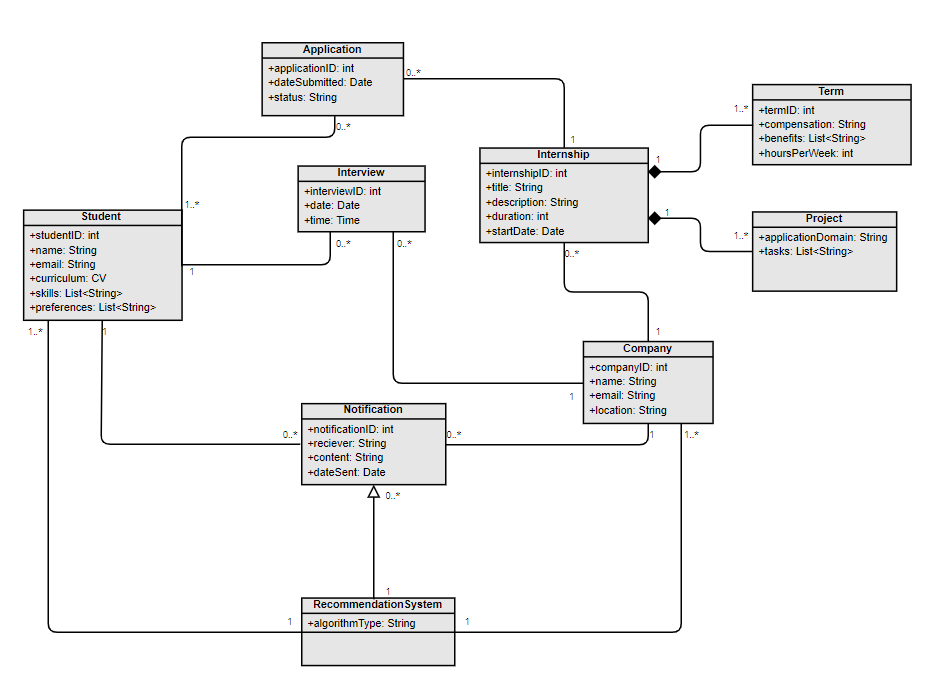
\includegraphics[scale=0.62]{rasd_diagrams/Class-Diagram.png}
    \caption{Students\&Companies (S\&C) Platform's domain class diagram}
    \label{fig:domain_class_diagram}
\end{figure}

\vspace{3cm}

The domain class diagram shown in Figure~\ref{fig:domain_class_diagram} illustrates the key entities and relationships in the S\&C platform. S\&C allows students and companies to interact similarly throughout the whole process of internships, right from the stage of application to selection.

\paragraph{Key Entities and Relationships:}
\begin{itemize}
    \item \textbf{Student}: Represents users searching for internships. Students can upload CVs, search for internships, and interact with companies. Each student profile includes unique attributes such as skills, preferences, and contact information.
    \item \textbf{Company}: Represents companies offering internships. Companies can advertise roles, review applications, and manage interviews through the platform. Each company profile includes details about the internship they are offering.
    \item \textbf{Internship}: Describes the specific roles offered by companies, including tasks, required skills, and terms of the position.
    \item \textbf{Project}: Specifies the technical and functional details of an internship, including technologies and domains.
    \item \textbf{RecommendationSystem}: Implements intelligent matching between students and internships by analyzing profiles, requirements and feedback.
    \item \textbf{Notification}: Handles alerts sent to both students and companies, informing them about matches, updates, and other events.
    \item \textbf{Application}: Tracks each student’s application to an internship, including its status (e.g., submitted, under review, accepted).
    \item \textbf{Interview}: Manages the scheduling and execution of interviews, including sharing structured questionnaires or other resources.
\end{itemize}

This diagram shows how a combination of different processes will work to buffer the students with companies by providing an orderly application progress for internships in a clear manner.


\newpage

\subsubsection{State Diagrams}

In this subsection, a discussion is provided regarding the state charts diagram for the internship application process. This diagram is essential for understanding the various states and transitions involved in managing the life cycle of an internship application.

\vspace{2cm}
\textbf{\footnotesize{Internship Application Management}} 
\vspace{0.1cm}

\begin{figure}[H]
    \centering
    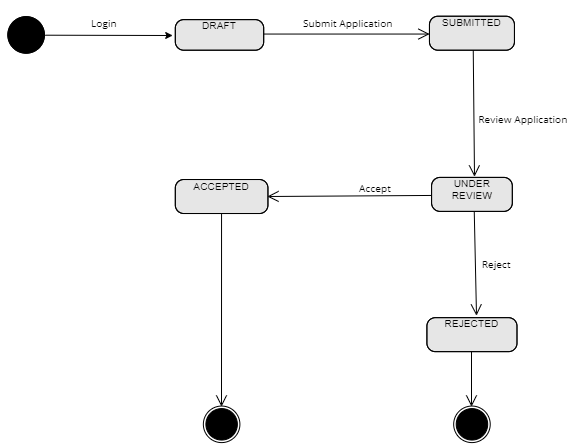
\includegraphics[scale=0.8]{rasd_diagrams/InternshipStateDiagram.png}
    \caption{Internship Application Process State Diagram}
    \label{fig:internship_state_chart}
\end{figure}

In this state charts diagram, the different states and transitions involved in the internship application process are represented. The process begins when a student logs into the platform, initiating the state of \textbf{Draft}, where they can prepare their application. The \textbf{Submitted} state is reached after the student submits their application.

Once submitted, the application moves to the \textbf{Under Review} state, where the company evaluates it. At this stage, two possible transitions exist: if the company rejects the application, it moves to the \textbf{Rejected} state, otherwise it moves to the \textbf{Accepted} state, where an internship is scheduled.

The process ends when the application reaches either the \textbf{Accepted} or \textbf{Rejected} state, with both being terminal states in the diagram.

\vspace{2cm}
\textbf{\footnotesize{Interview Application Management}} 
\vspace{0.1cm}

\begin{figure}[H]
    \centering
    
\includegraphics[scale=0.8]{RASD/rasd_diagrams/InterviewStateDiagram.png}
    \caption{Interview Application Process State Diagram}
    \label{fig:interview_state_chart}
\end{figure}

In this state chart, diagrams represent the different states that an interview process can reach.\\
The process begins when an application is accepted, initiating the process \textbf{Scheduled}, where the student who submitted the application, sending him questionnaires and evaluating his responses. 
The process continues until the company has not taken a decision, after which two outcomes are possible. 
If the interview is successful, the interview transitions to the \textbf{Hired} state, signifying that the student has secured the internship. In contrast, if the company decides not to proceed, the interview transitions to the \textbf{Refused} state.
The process ends when the interview reaches the \textbf{Hired} or \textbf{Refused} state, both terminal states in the diagram.


\newpage

\subsection{Product Functions}

\subsubsection{Sign-up and Log-in}
This function is available to all users who want to subscribe to the platform. When a new user opens the platform, they can press the button 'Sign-up'. The system then redirects the user to the registration page, where they can create an account by providing their email, username, and password. Once the account is created, the user can log in to the platform with their credentials to access the system functions.

\subsubsection{Internship Management by Companies}
This function allows companies to manage internship opportunities. After logging in, a company can create an internship by filling out a form specifying the internship’s application domain, tasks to be performed, technologies, and terms offered. Companies can also edit or delete their published internships based on their evolving needs.

\subsubsection{CV Management by Students}
This function allows students to upload their CVs. Once logged into the platform, students are directed to a section where they can fill in their skills, experiences, and educational background to generate a CV. Students can update or replace their CVs whenever necessary to reflect their most recent achievements. The platform ensures that uploaded CVs are visible to companies searching for suitable candidates.

\subsubsection{Search and Application for Internships}
This function allows students to browse and search for internships posted by companies. Students can filter internships based on domains, tasks, technologies, or terms. Once a student identifies a suitable internship, they can submit their application. This application is stored in the platform and made available to the corresponding company for review.

\subsubsection{Recommendation System}
The platform integrates a recommendation system to simplify the internship matching process. For students, the recommendation system analyzes their uploaded CVs and preferences to suggest internships that align with their skills. On the other hand, for companies, the system suggests students whose profiles meet their specified requirements. These recommendations are displayed as notifications, allowing both parties to evaluate and act on potential matches efficiently.

\subsubsection{Interview Scheduling and Management}
This function supports the interview process between students and companies. When a company is interested in a student’s application, they can use the platform to schedule an interview. The system provides tools for managing the interview, such as setting dates and sharing structured questionnaires. Notifications about scheduled interviews are sent to both students and companies, ensuring effective communication and coordination.

\subsubsection{Application Status Tracking}
Students can track the status of their internship applications through this function. Applications transition between states such as \textit{Submitted}, \textit{Under Review}, \textit{Accepted}, and \textit{Rejected}. These status updates are visible on the student’s dashboard, providing real-time insights into their application progress.

\subsubsection{Internship Acceptance and Finalization}
Once the interview process concludes, companies can accept or reject applications. Accepted applications transition to a finalized state, and the student receives an offer notification. This function ensures that both parties have clear and structured communication regarding the outcome, marking the official start of the internship.

\subsubsection{Feedback Collection and Analysis}
This function lets users give feedback about their time on the platform. Students can rate the internships they did and write some comments if they want to share more about their experience. Companies can also give feedback on the students they worked with, saying what they thought about them during the internship.
The platform takes this feedback and uses it to improve how it recommends matches in the future. It helps make better suggestions for both students and companies.


\newpage

\subsection{2.3 User Characteristics}

There are two main types of users that interact with the platform: students and companies.

\subsubsection{Student}
A student is able to register and log in to the platform. Students can search for internships, upload their CVs, and participate in the recommendation and selection process. They can also be notified by the system when internships matching their profiles become available.

\subsubsection{Company}
A company is a user that advertises internships on the platform. Companies can create internship offers, review student applications, and manage the selection process, including scheduling interviews. They also receive notifications when suitable candidates are identified by the system.

\subsection{Assumption, Dependencies and Constraints}
    The following assumptions are made for the domain and taken for granted by the system.They must be verified to ensure the correct platform behavior.
    The domain assumption for S\&C are:
    \begin{itemize}
        \item \textbf{[D1]} Users have a reliable internet connection.
        \item \textbf{[D2]} Students do not lie when compiling his resume.
        \item \textbf{[D3]} Companies do not insert false information in their advertise.
        \item \textbf{[D4]} Students and companies give a truthful feedback at the end of their internship experience.
        \item \textbf{[D5]} Students answer to questionnaires sent by the companies during the selection process.
    \end{itemize}
    

\newpage

\section{Specific Requirements}

\subsection{External Interface Requirements}

\subsubsection{User Interfaces}

The Students\&Companies platform provides an intuitive and user-friendly interface designed to meet the needs of its two primary stakeholders: students and companies. Below, we illustrate key aspects of the interface design for different user roles.

\begin{figure}[H]
    \centering
    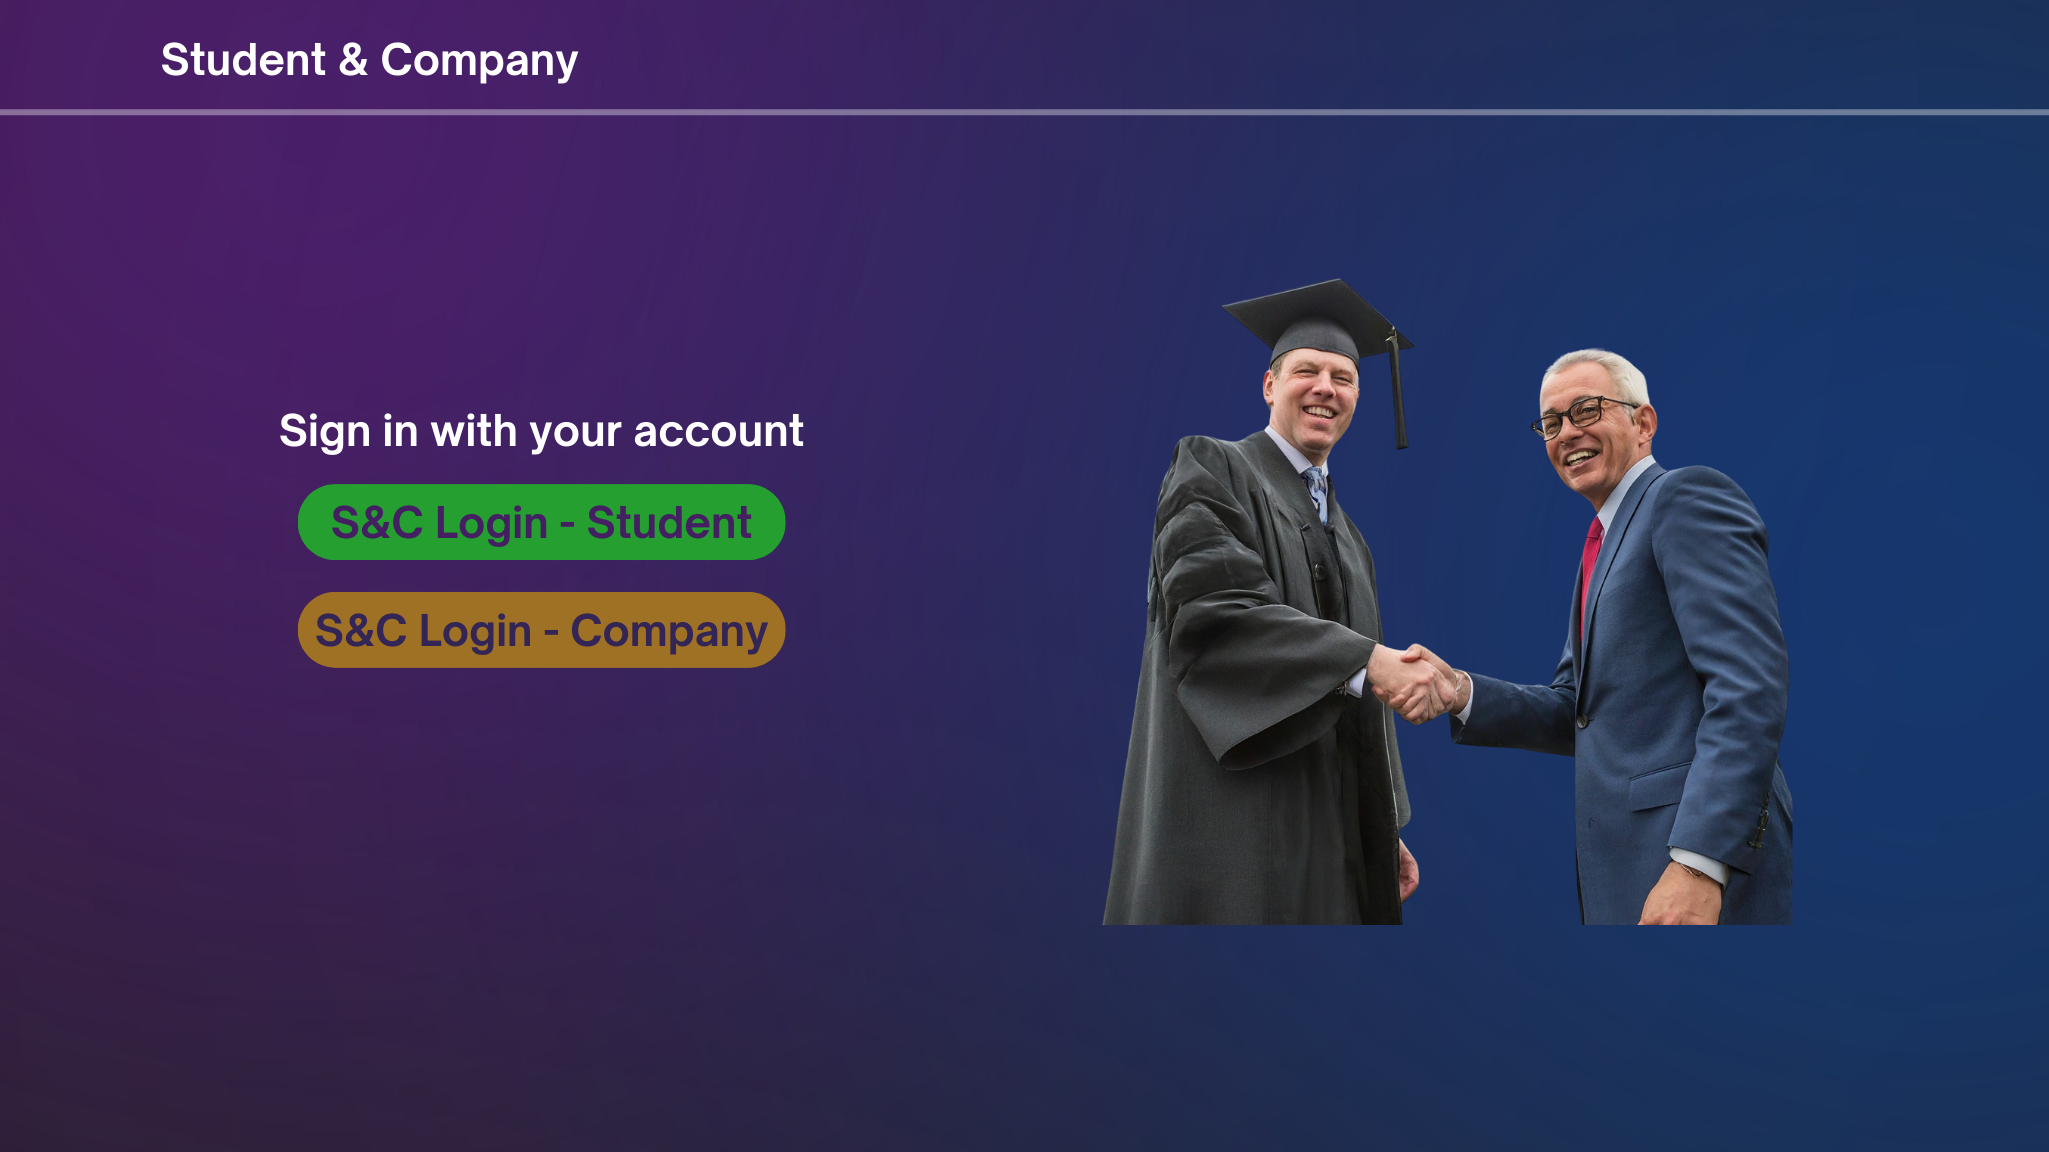
\includegraphics[width=\textwidth]{design png/1.png}
    \caption{Login Page}
    \label{fig:login_page}
\end{figure}

\begin{figure}[H]
    \centering
    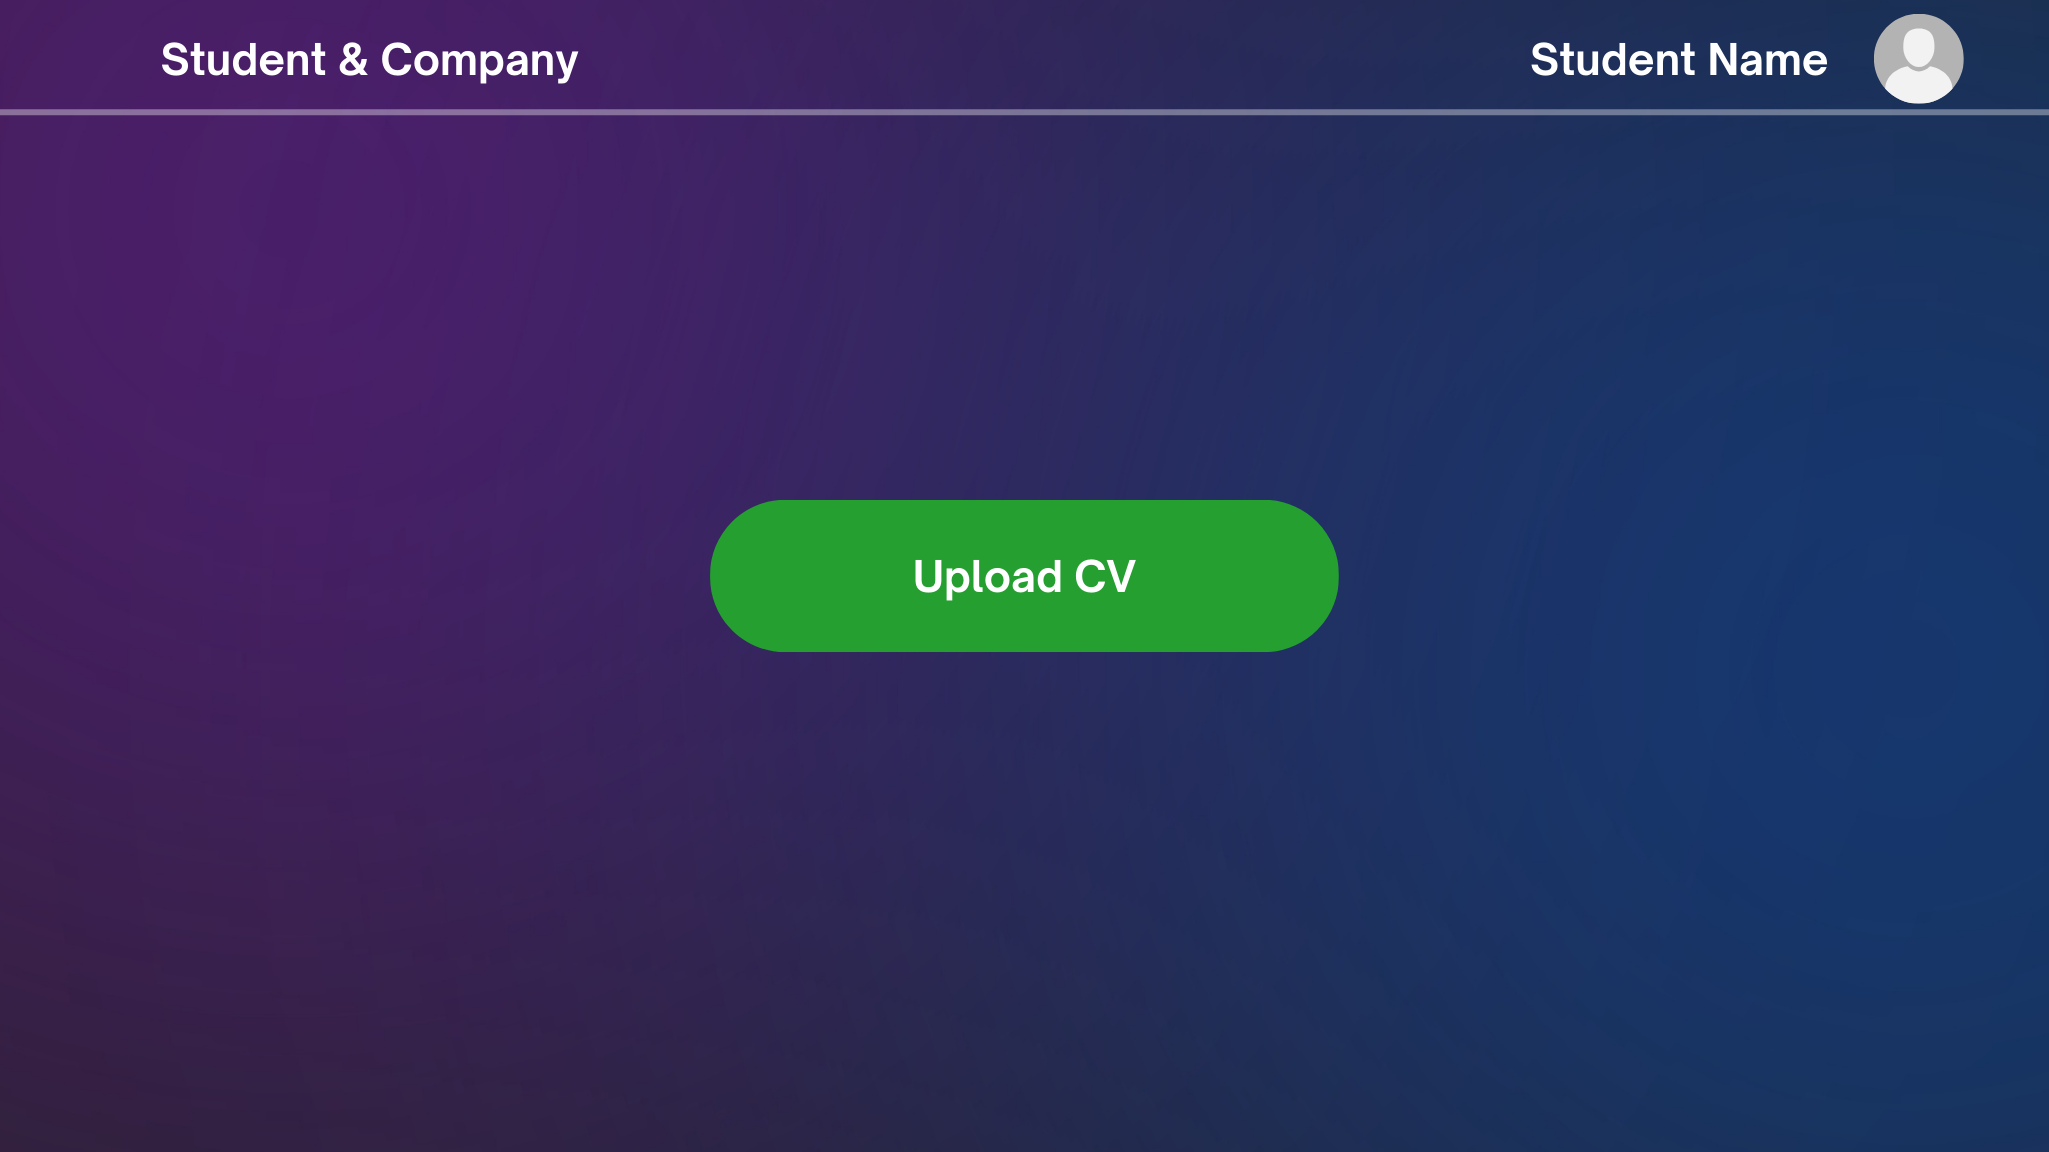
\includegraphics[width=\textwidth]{design png/2.png}
    \caption{CV Upload Page}
    \label{fig:cv_upload_page}
\end{figure}

\begin{figure}[H]
    \centering
    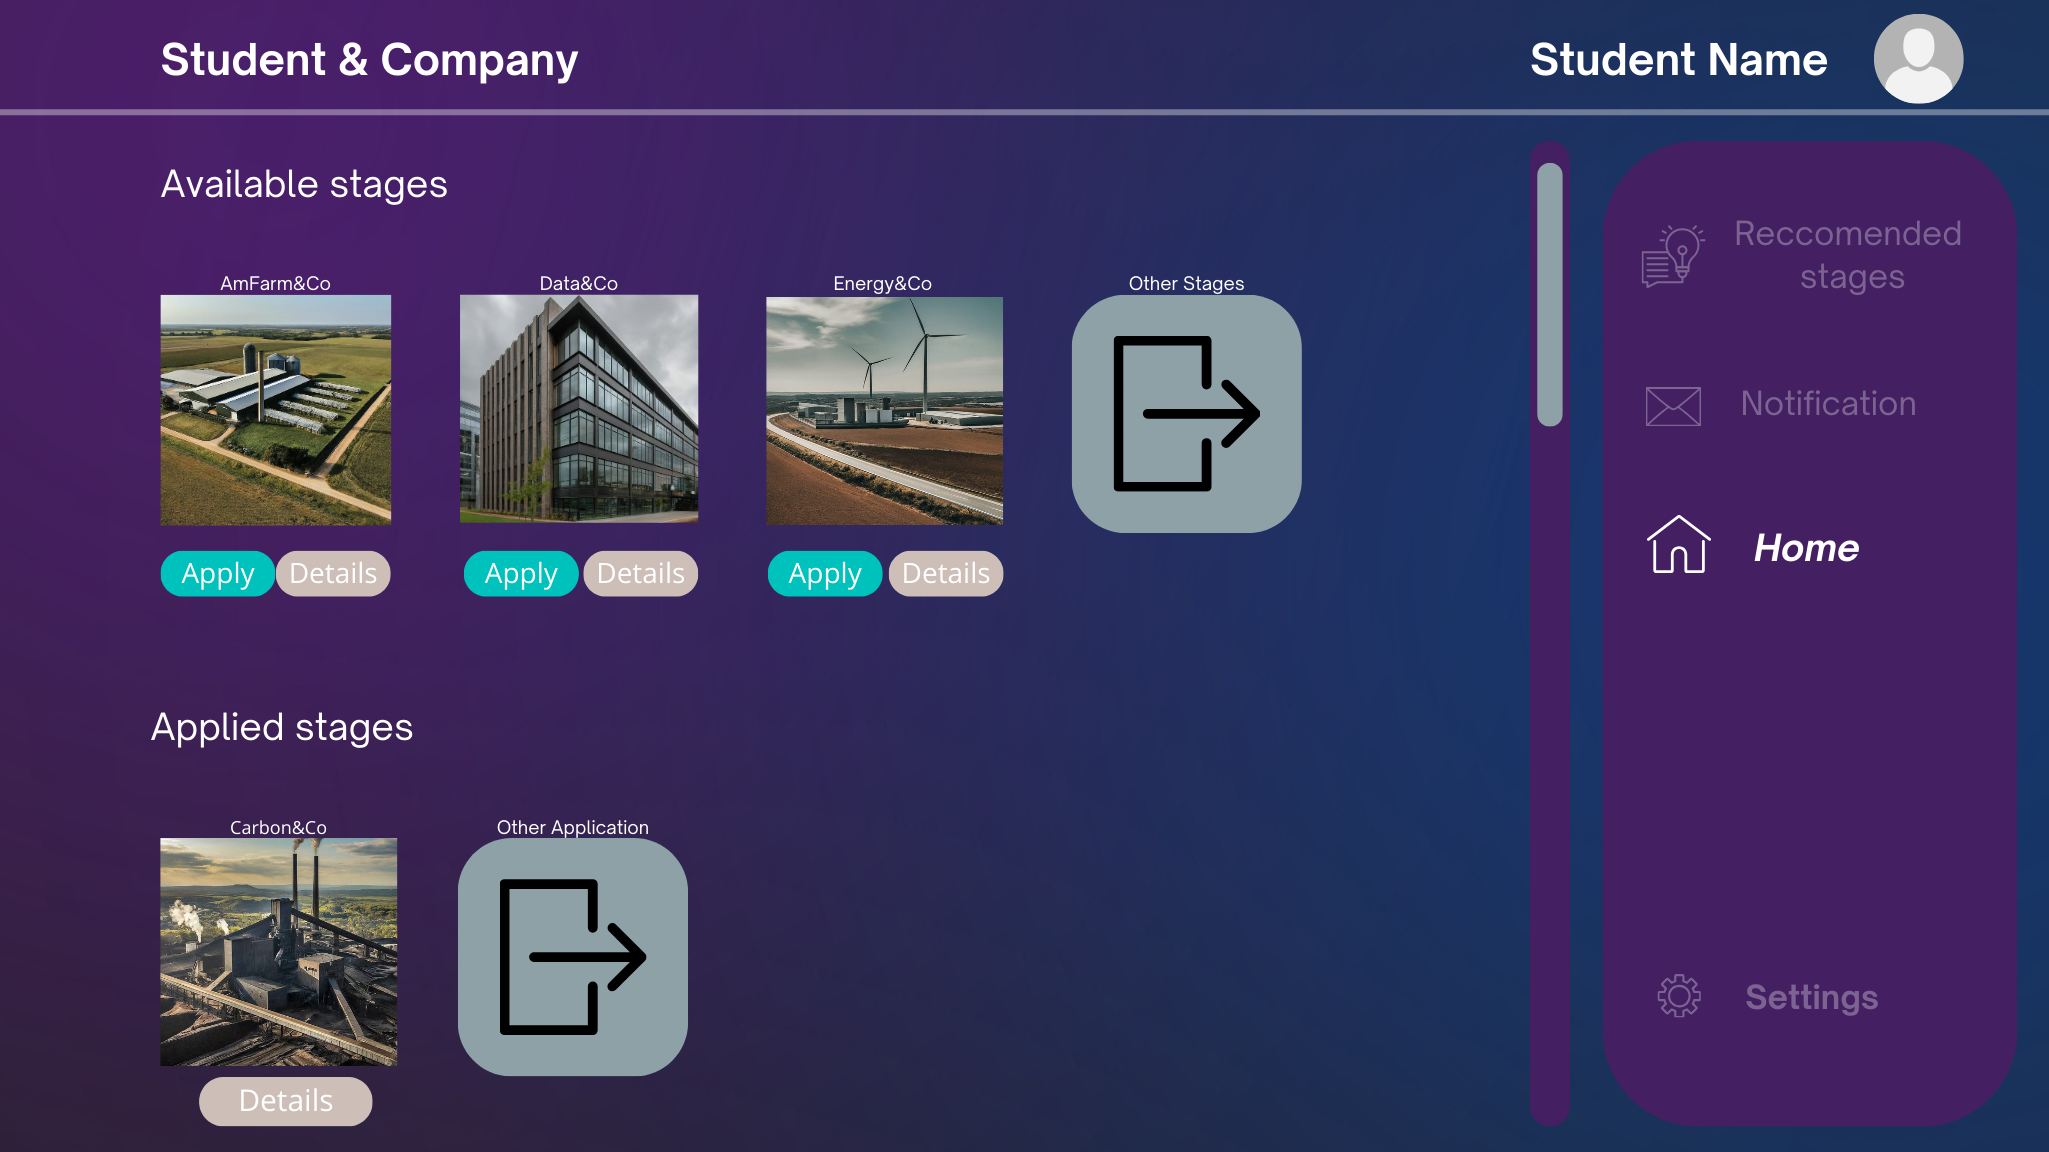
\includegraphics[width=\textwidth]{design png/3.png}
    \caption{Student Home Page}
    \label{fig:student_dashboard}
\end{figure}

\begin{figure}[H]
    \centering
    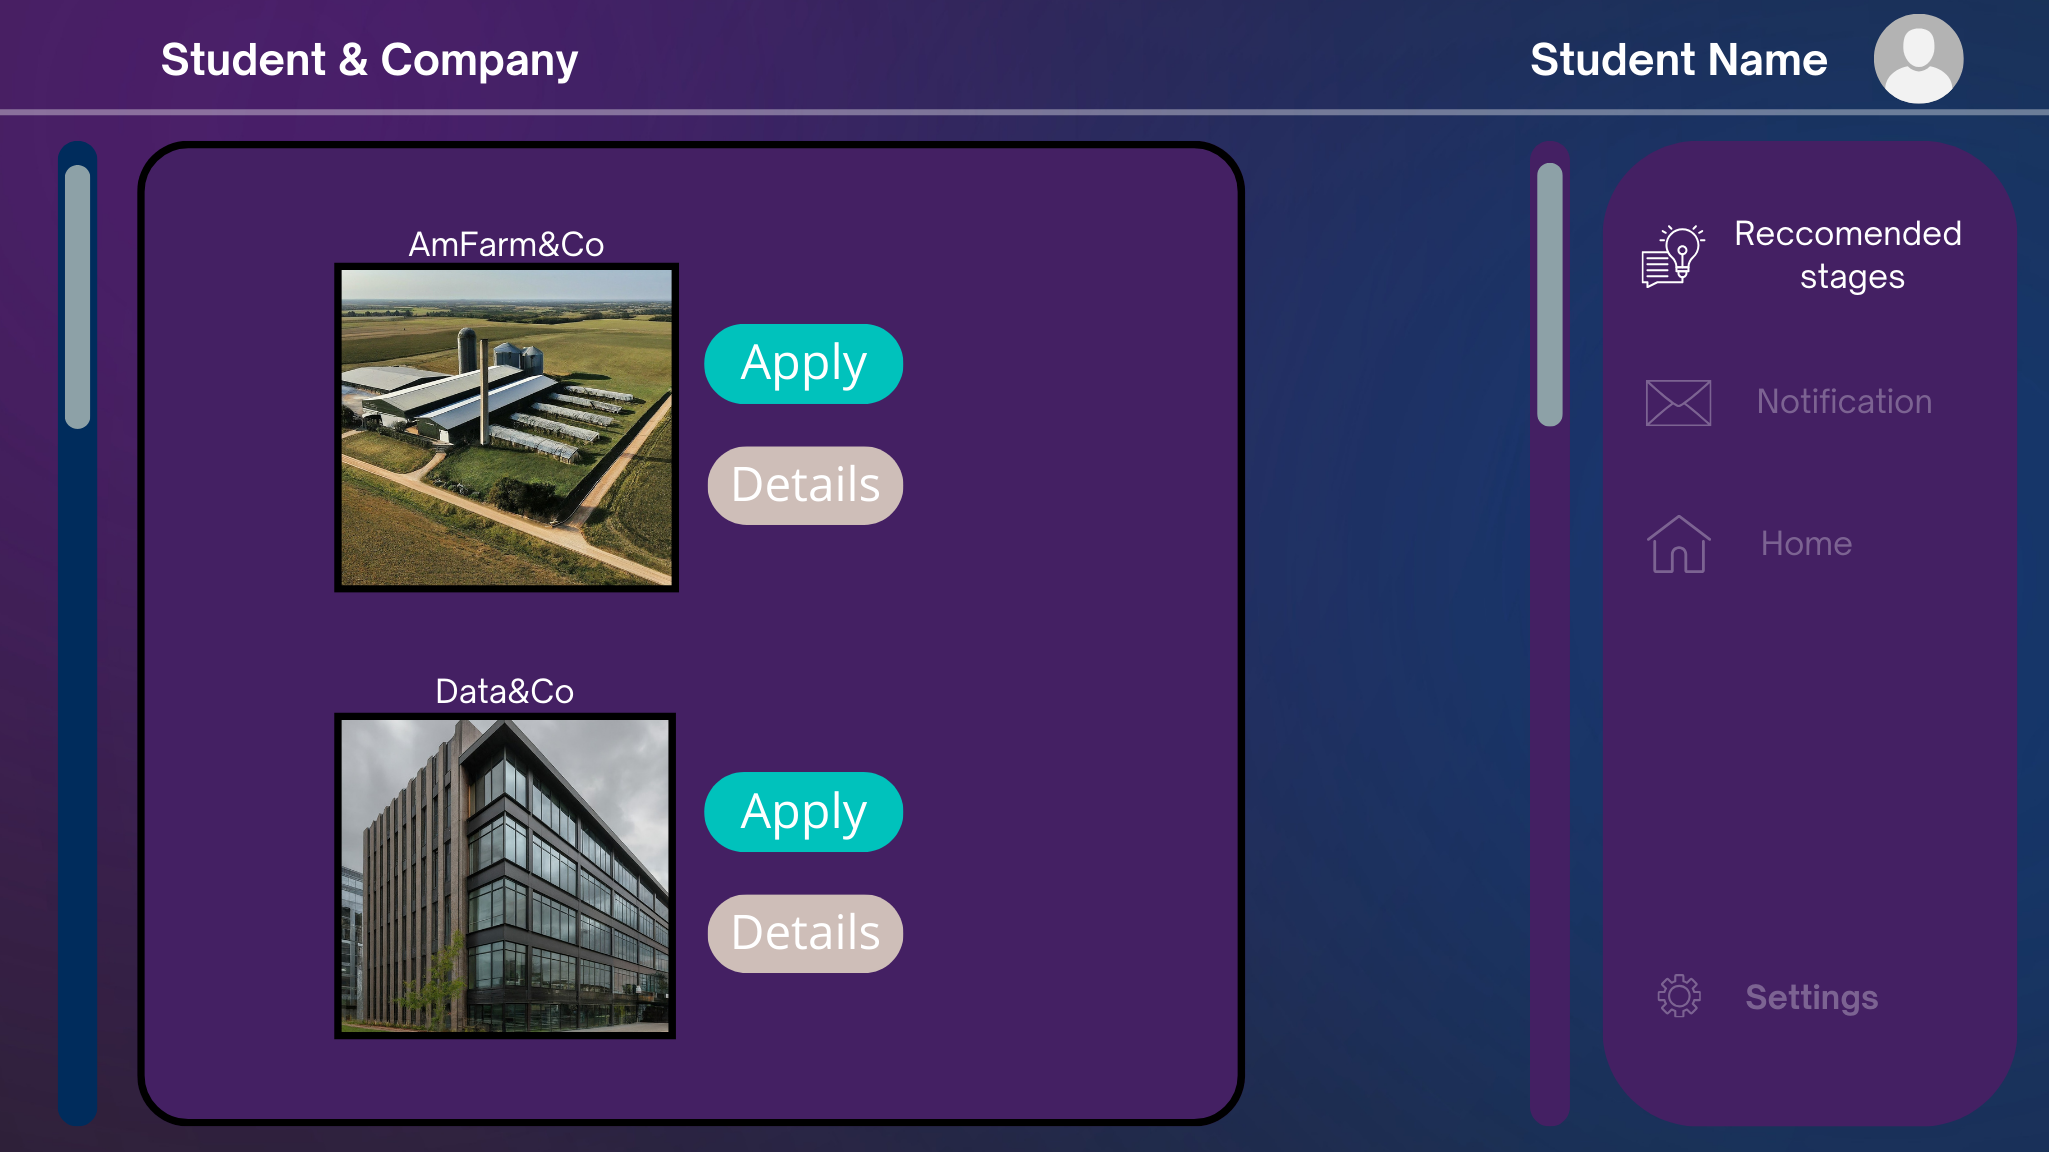
\includegraphics[width=\textwidth]{design png/4.png}
    \caption{Recommended Stages Page}
    \label{fig:student_home_page}
\end{figure}

\begin{figure}[H]
    \centering
    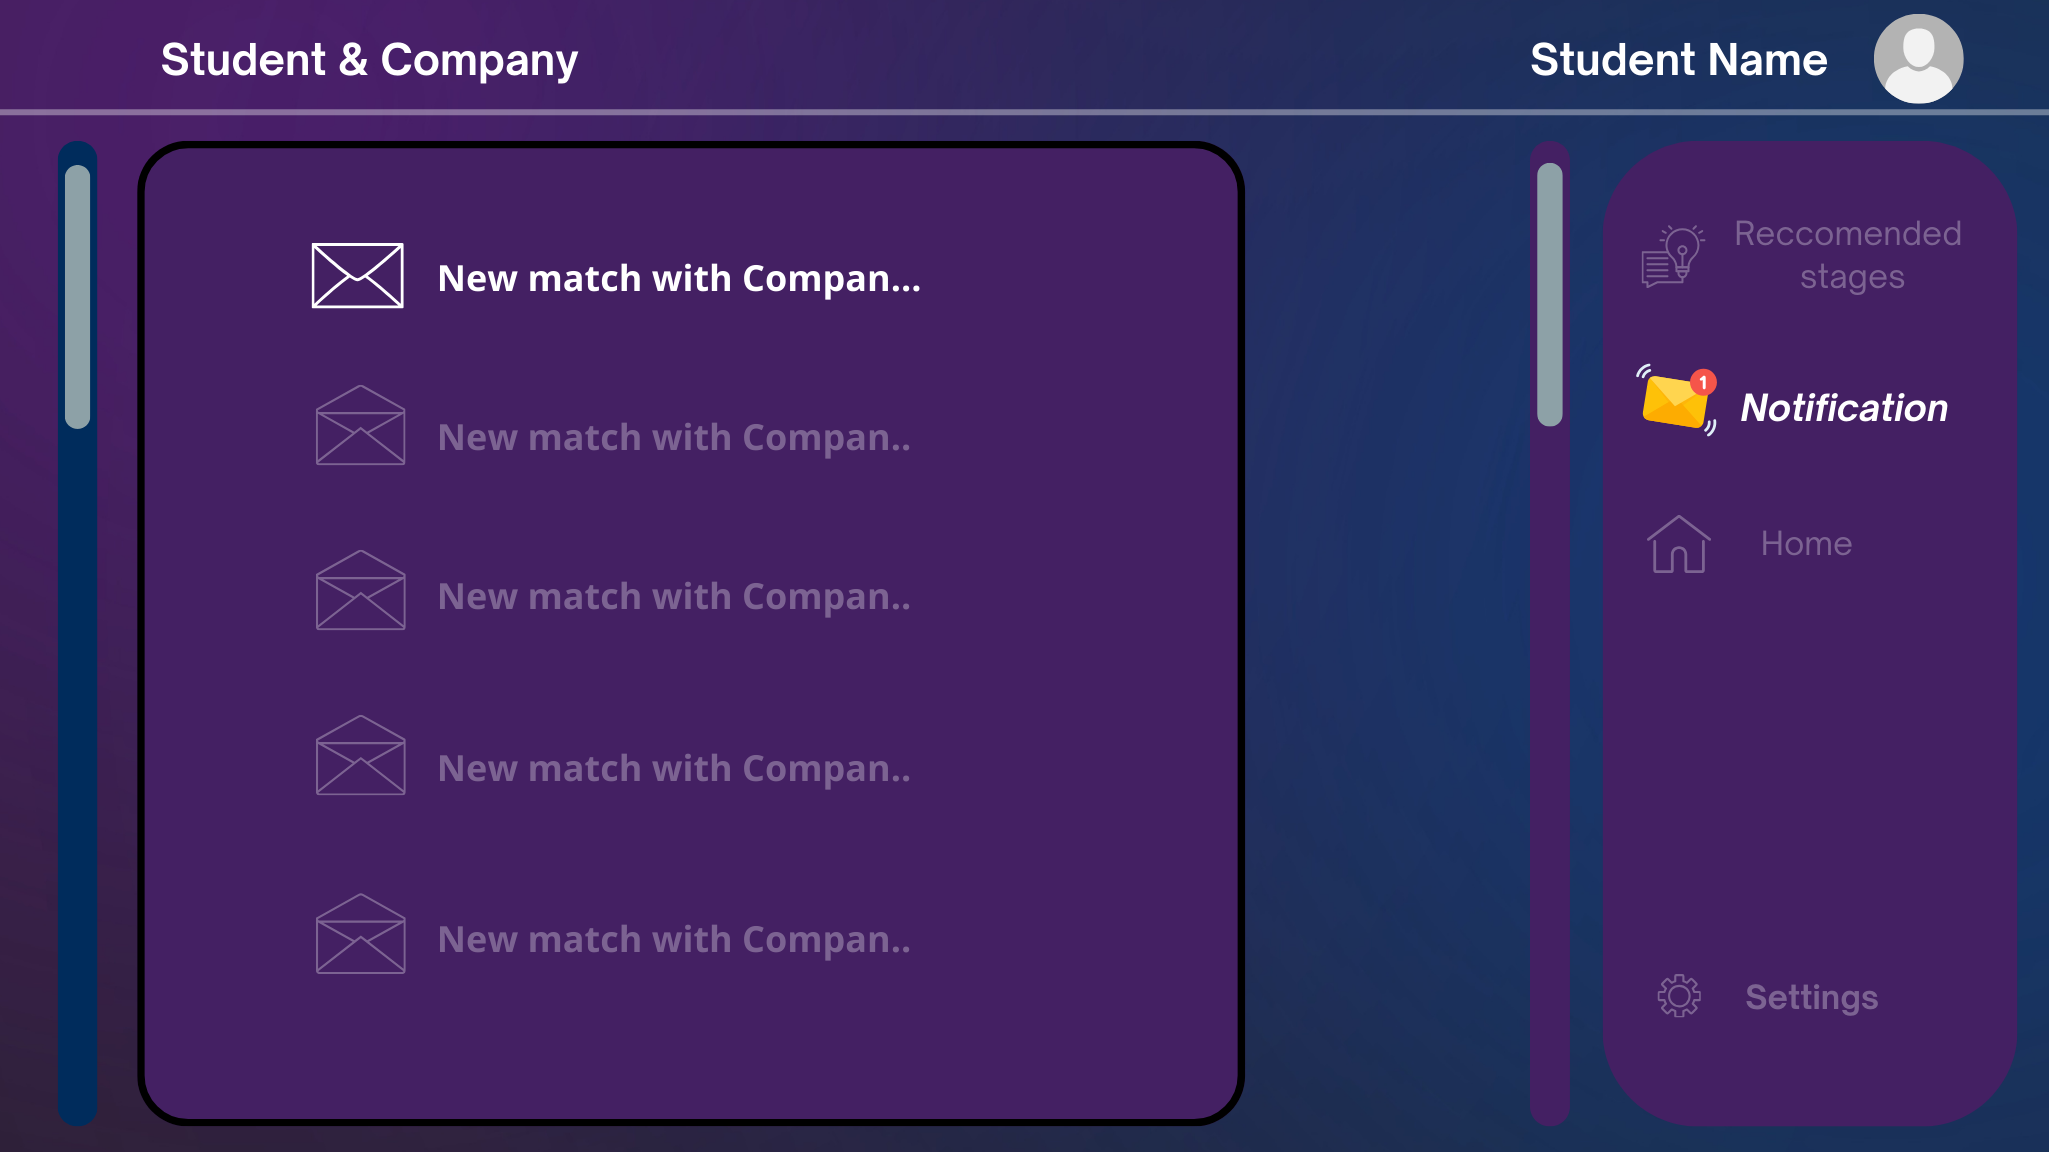
\includegraphics[width=\textwidth]{design png/5.png}
    \caption{Notification Center:}
    \label{fig:recommended_stages}
\end{figure}

\begin{figure}[H]
    \centering
    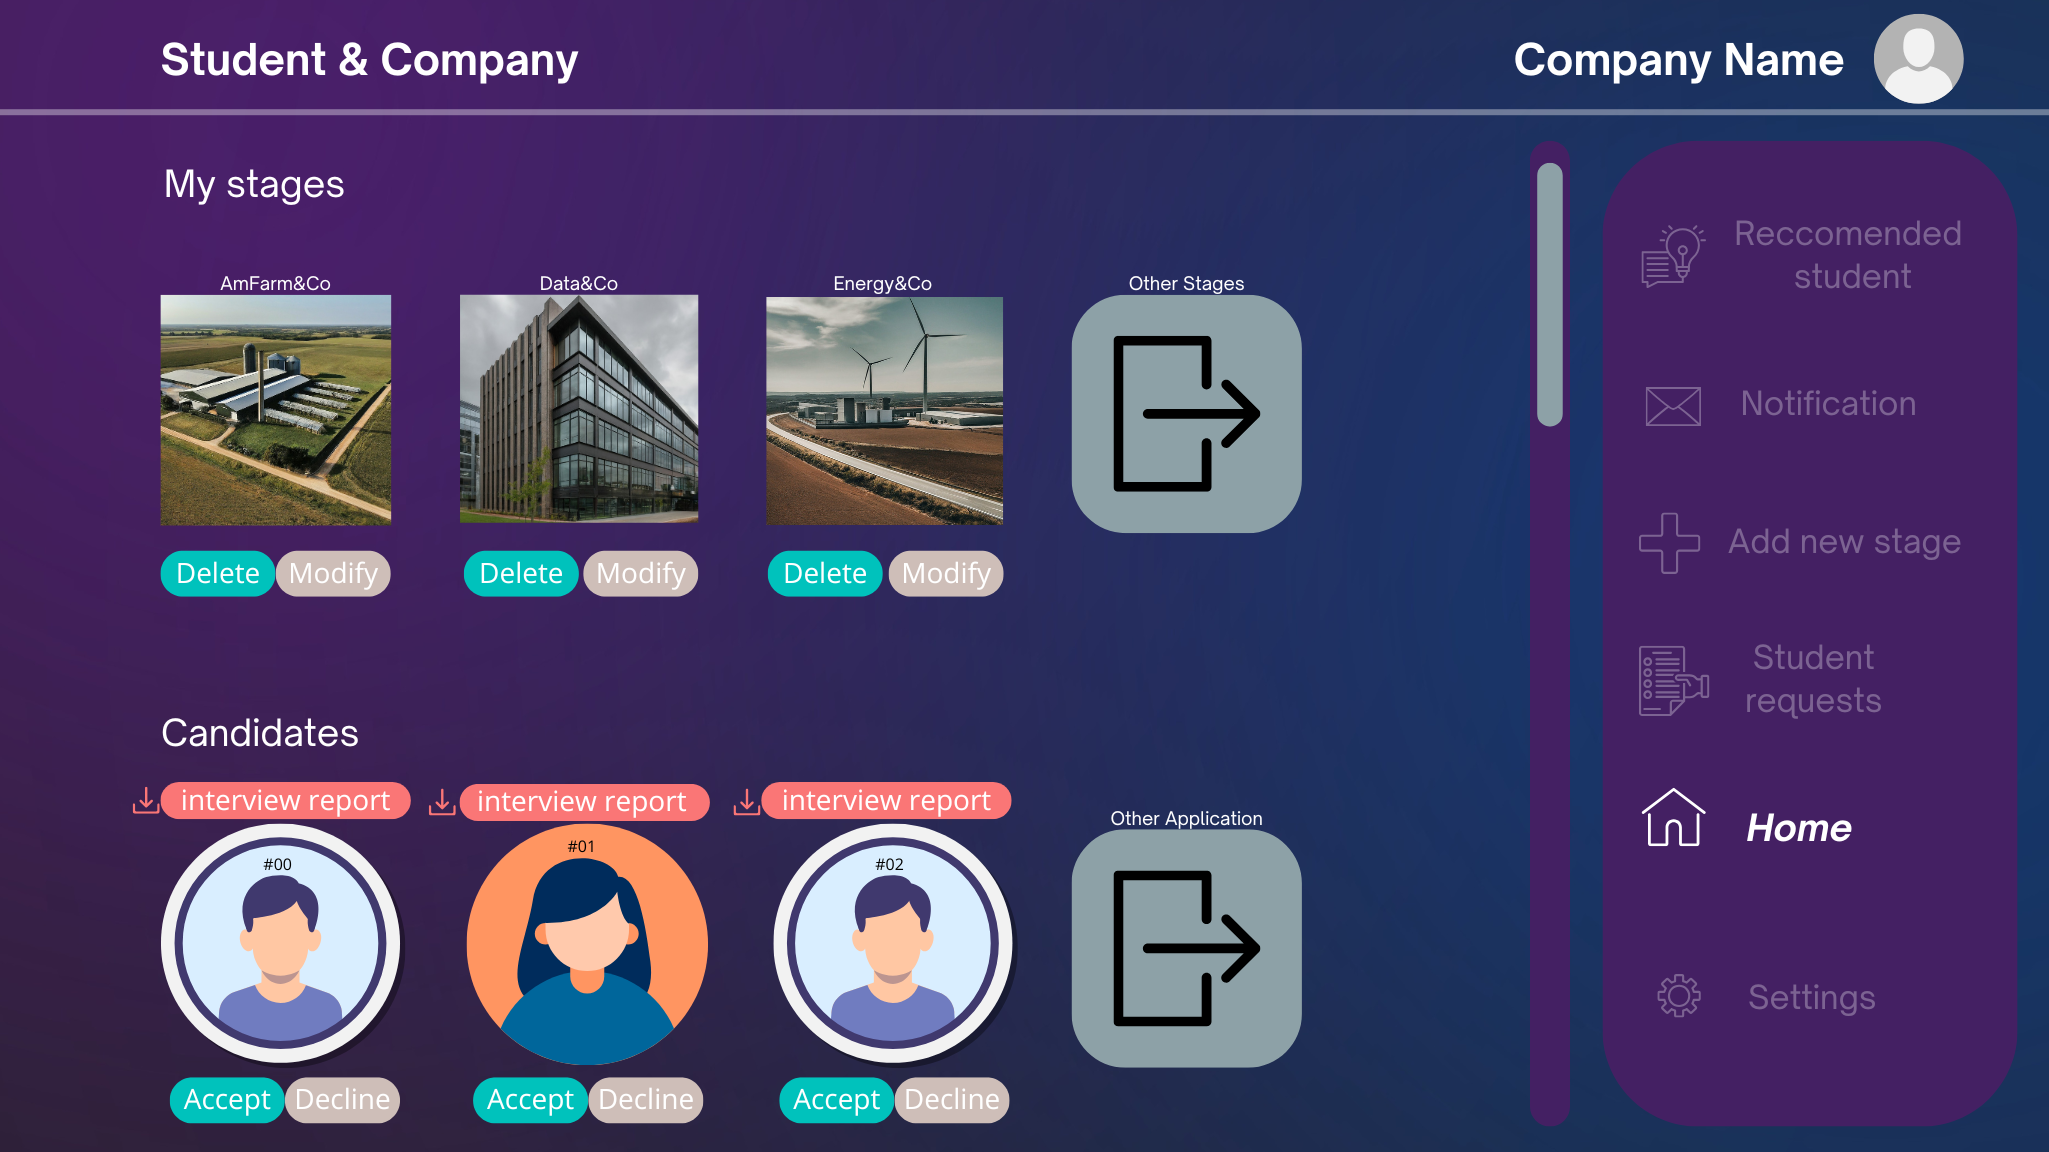
\includegraphics[width=\textwidth]{design png/6.png}
    \caption{Company Home Page:}
    \label{fig:notification_center}
\end{figure}

\begin{figure}[H]
    \centering
    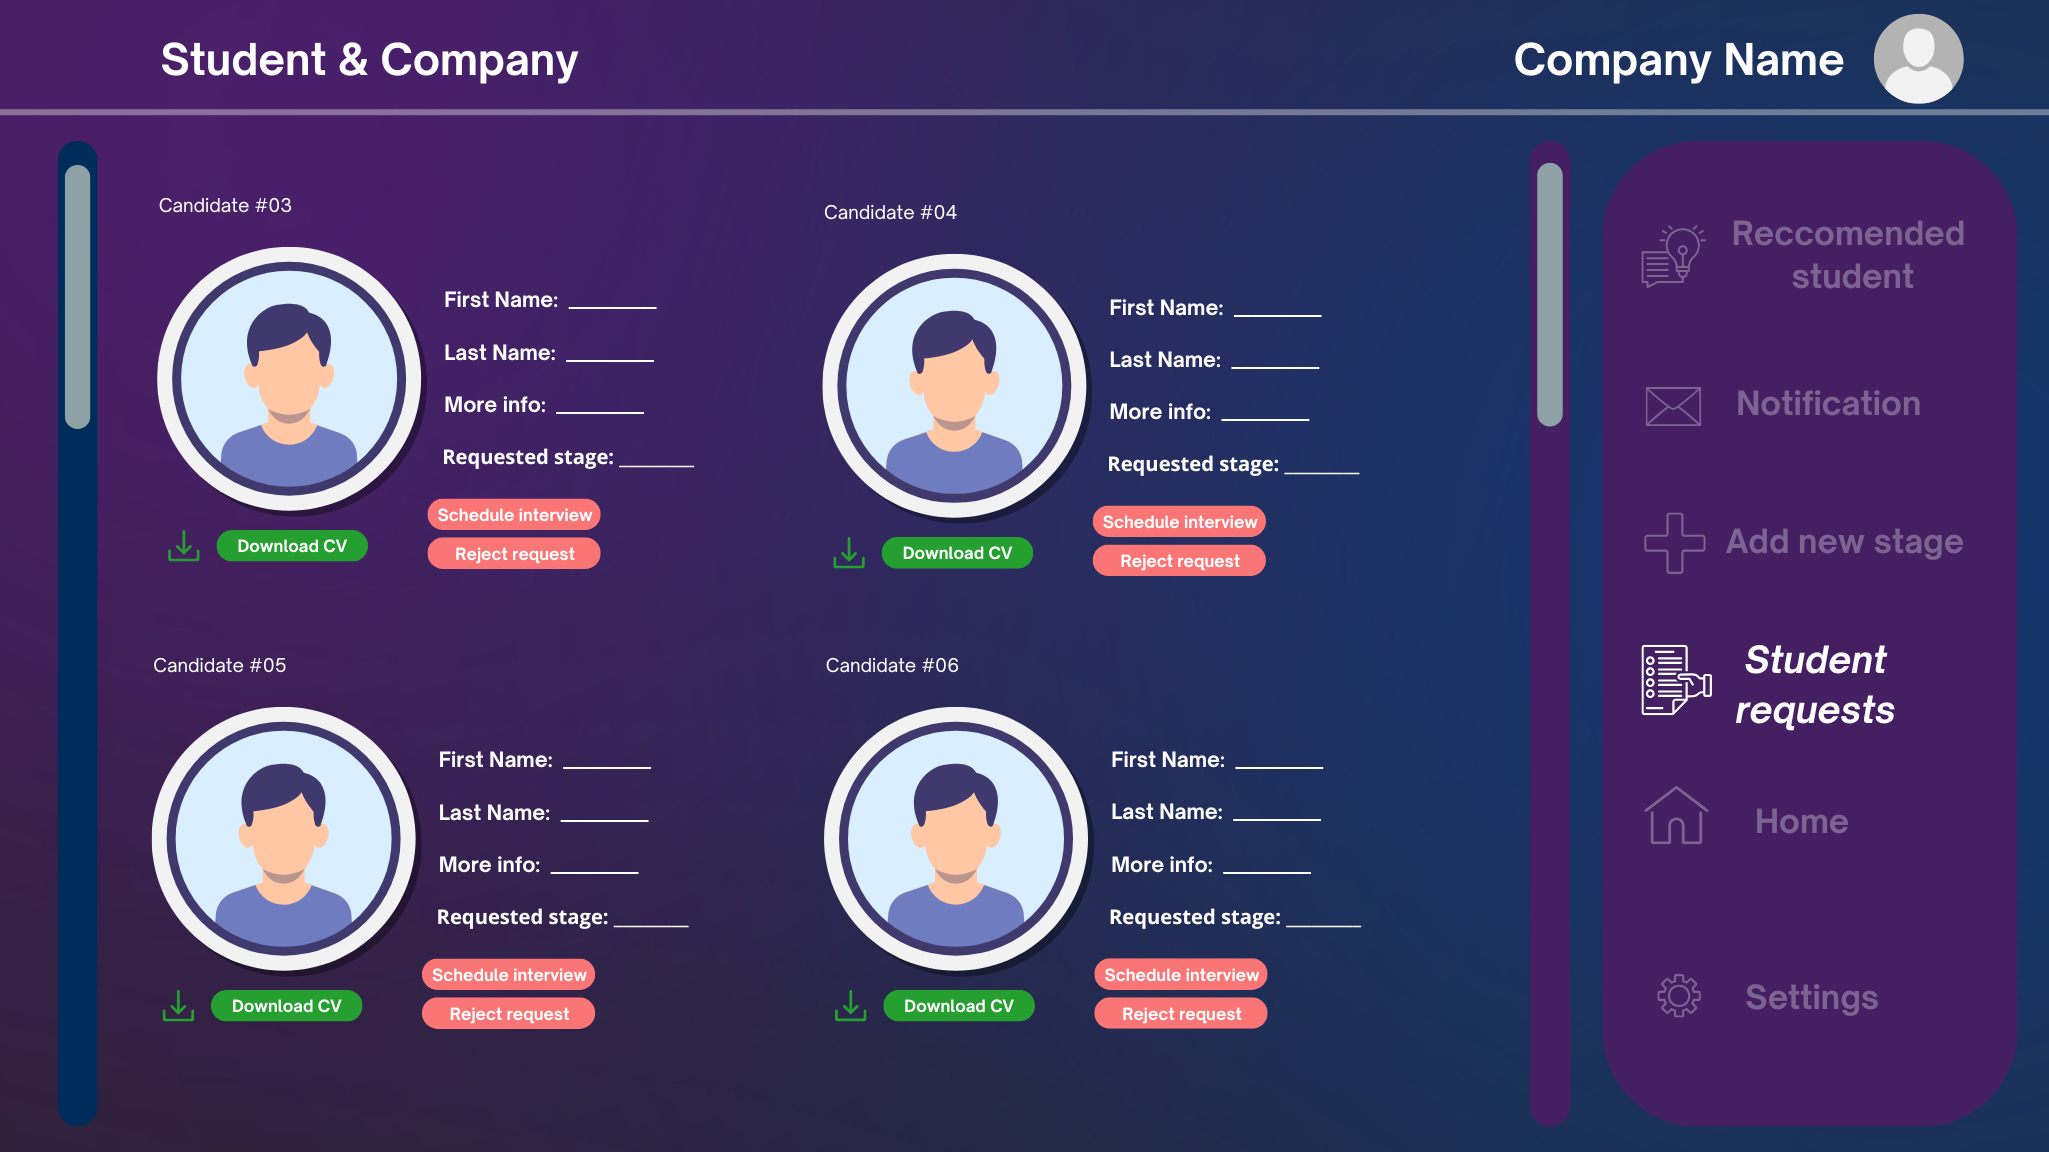
\includegraphics[width=\textwidth]{design png/7.png}
    \caption{Candidate Management Page:}
    \label{fig:company_home_page}
\end{figure}

\begin{figure}[H]
    \centering
    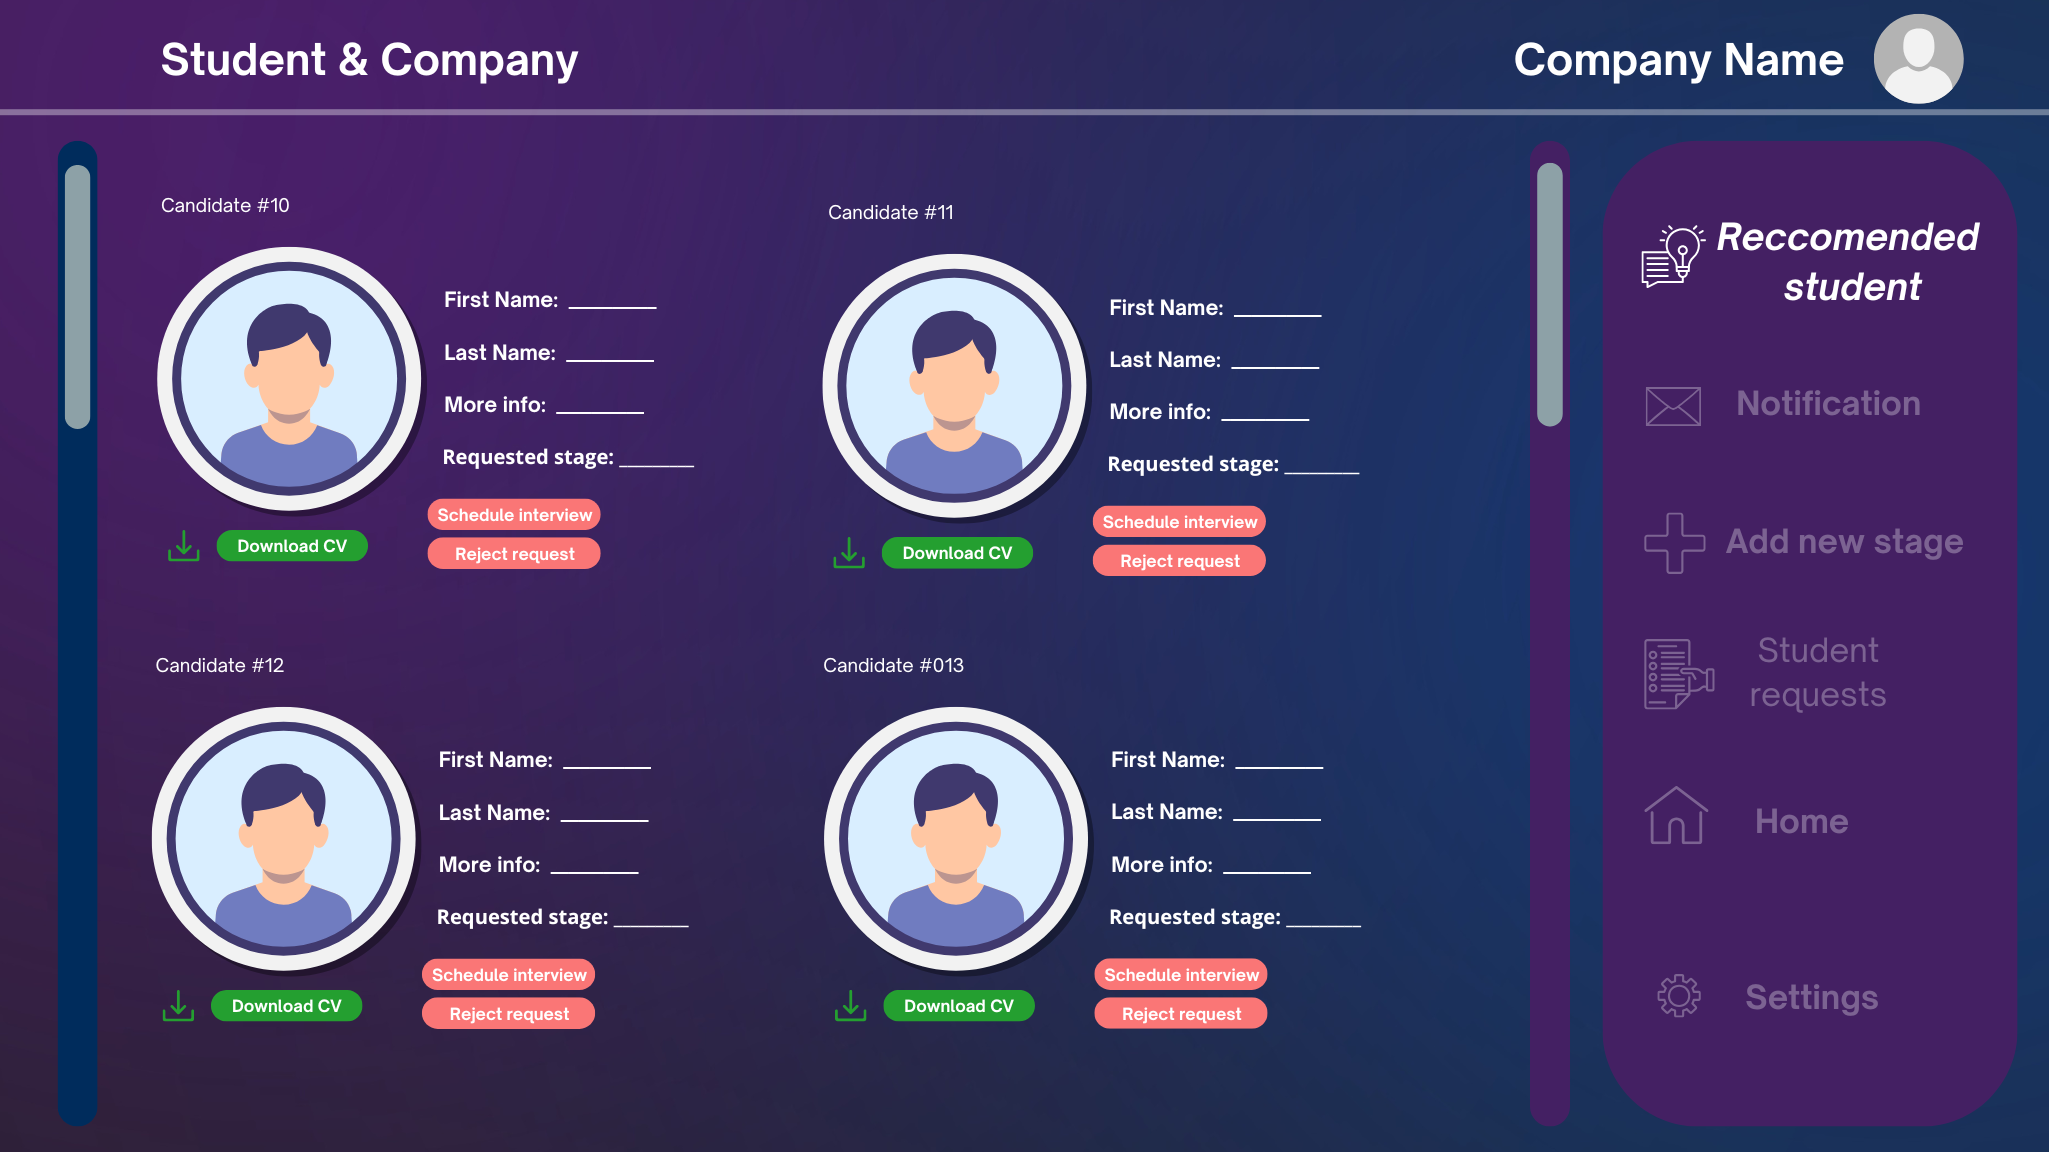
\includegraphics[width=\textwidth]{design png/8.png}
    \caption{Recommended Students Page:}
    \label{fig:candidate_management}
\end{figure}

\begin{figure}[H]
    \centering
    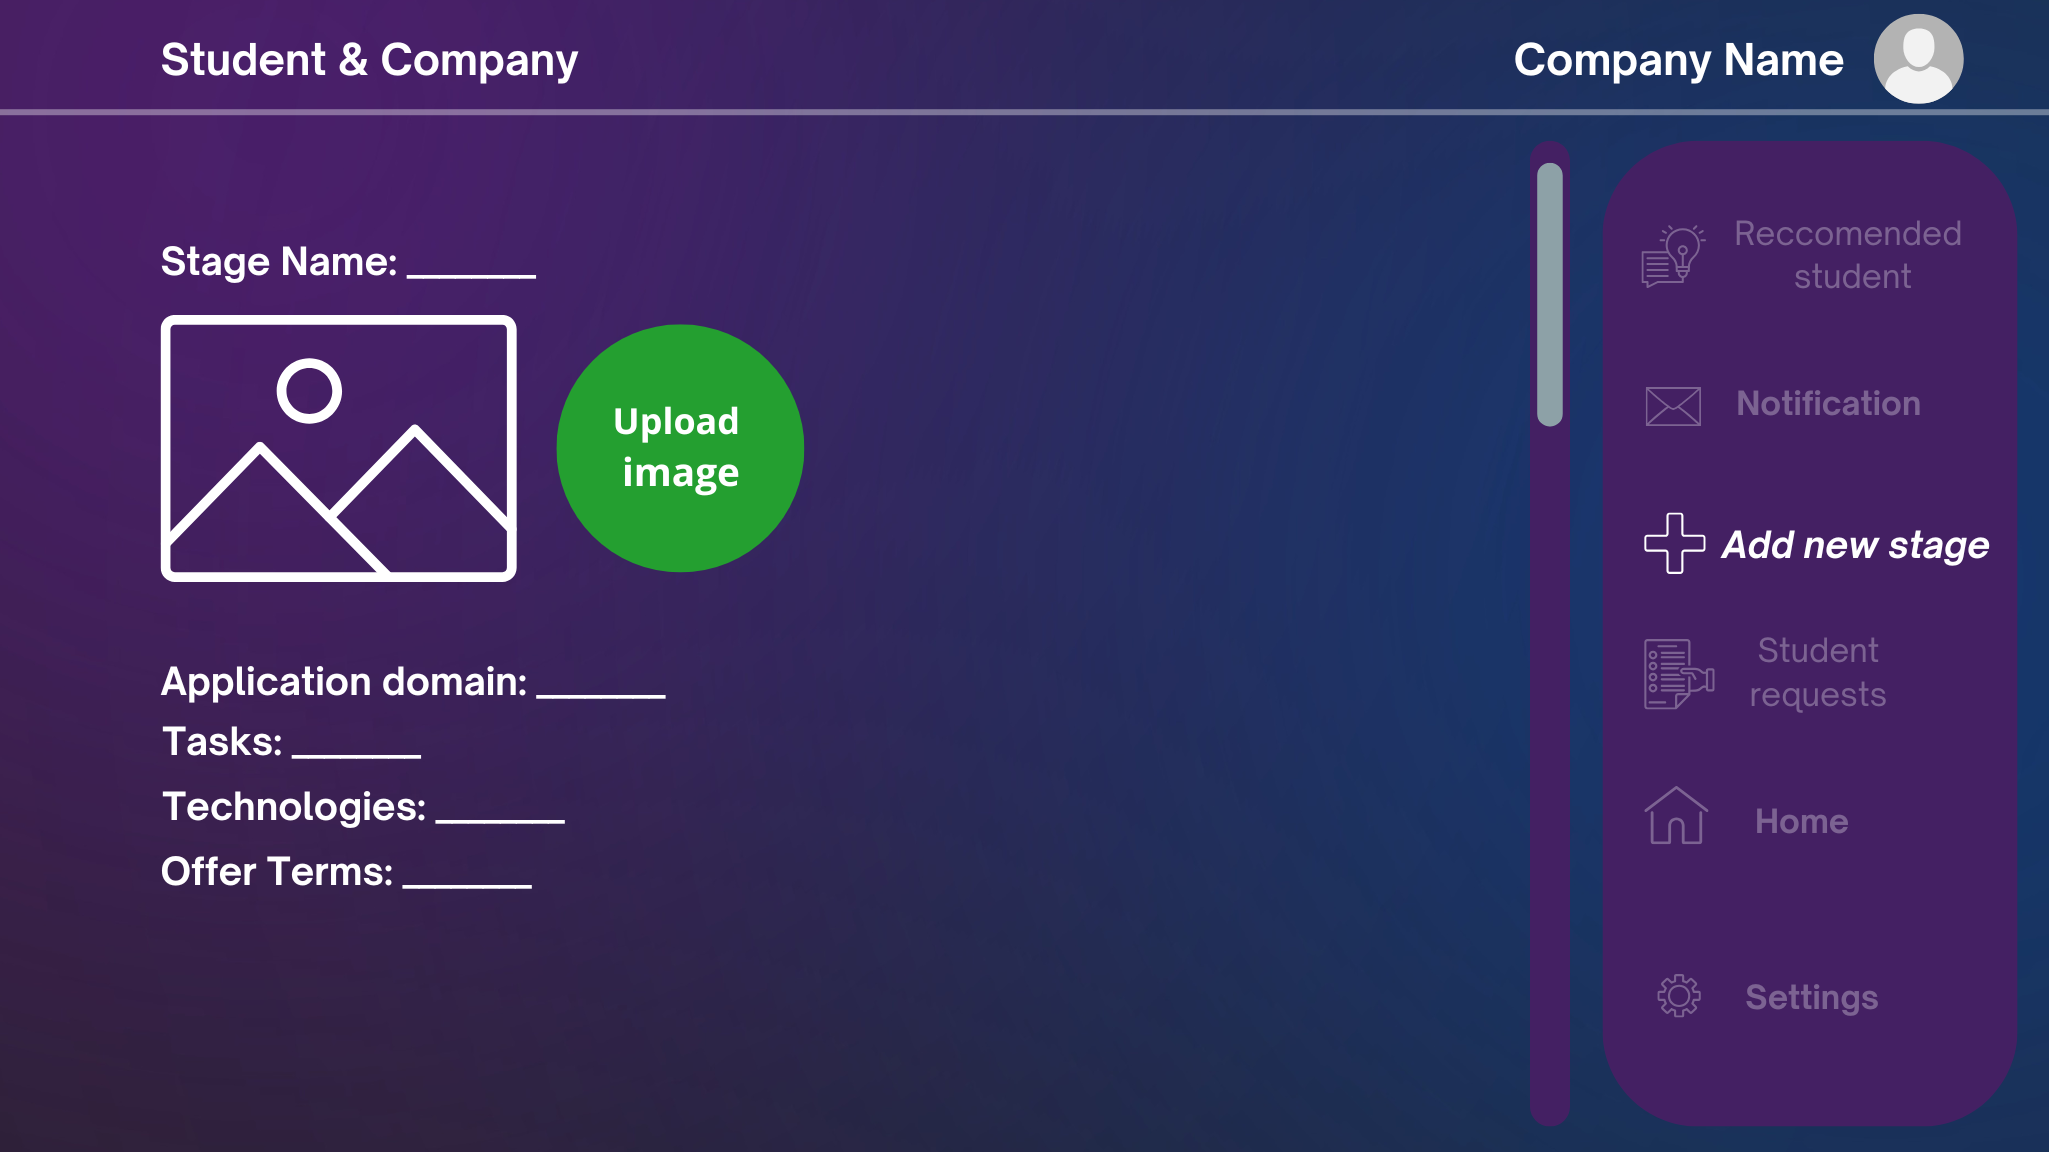
\includegraphics[width=\textwidth]{design png/9.png}
    \caption{New Stage Creation Page}
    \label{fig:recommended_students}
\end{figure}

\begin{figure}[H]
    \centering
    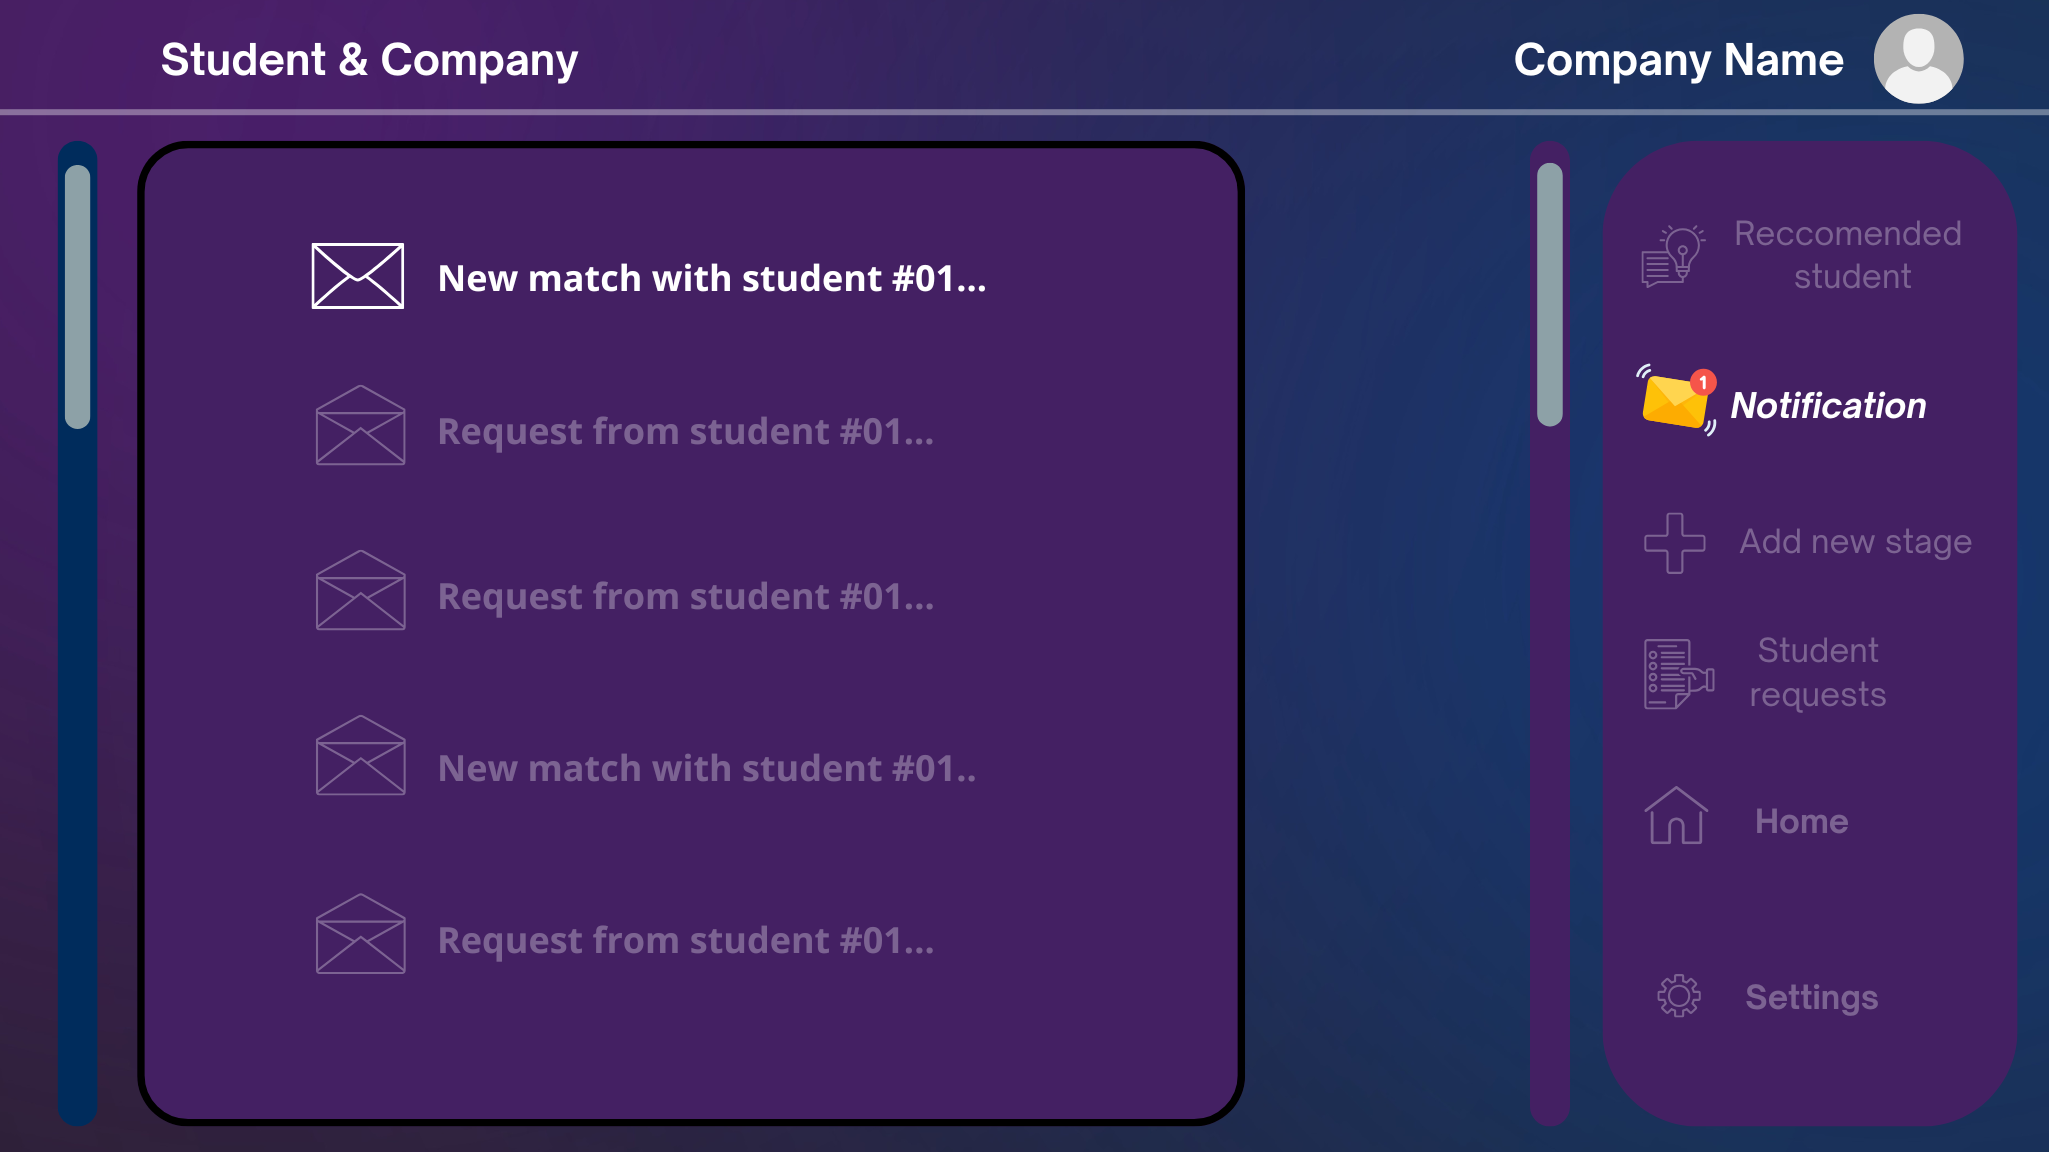
\includegraphics[width=\textwidth]{design png/10.png}
    \caption{Company Notification Page}
    \label{fig:new_stage_creation}
\end{figure}

\newpage


\subsubsection{Hardware Interfaces}
    Since the system won't interact with any particular external hardware, no remarkable constraints and hardware interfaces are needed.
    
\subsubsection{Software Interfaces}
    In order to guarantee part of its functionalities, S\&C needs the following software interface:
        \begin{itemize}
            \item \textbf{Recommendation System API}: this interface is used by S\&C to communicate with the recommendation system, which is needed to suggest students to companies and vice versa, through mechanism such as statistical analysis and keyword searching.
        \end{itemize}

\subsubsection{Communication Interfaces}
    The web app will communicate with S\&C via an internet connection. The communication protocols that will be used by the system is:
        \begin{itemize}
            \item \textbf{HyperText Transfer Protocol over Secure Socket Layer (HTTPS)}. This protocol is used every time an exchange of information with the external world is needed.
        \end{itemize}
        
\newpage
\subsection{Functional Requirements \& Goals - Requirement mapping}

    \begin{center}
        \begin{longtable}{|l|p{0.75\linewidth}|}
            \hline
            \multicolumn{2}{|p{0.75\linewidth}|}{\textbf{[G1] - Allows students and companies to register and log in, so that students can search and apply for an internship, while companies can evaluate proposals and interview students.}} \\
            \hline
            \textbf{ID} & \textbf{Requirement}  \\
            \hline
            \textbf{R1} & The system allows users to register to the platform. \\
            \hline
            \textbf{R2} & The system allows users to login to the platform through their credentials. \\
            \hline
            \caption{Goal 1 requirements}
        \end{longtable}
    \end{center}

    \begin{center}
        \begin{longtable}{|c|p{0.75\linewidth}|}
            \hline
            \multicolumn{2}{|p{0.75\linewidth}|}{\textbf{[G2] - Helps students and companies manage, respectively, resumes and internships.}} \\
            \hline
            \textbf{R3} & The system permits students to upload their CVs. \\
            \hline
            \textbf{R4} & The system permits students to modify their CVs. \\
            \hline
            \textbf{R5} & The system permits companies to publish their internship proposal. \\
            \hline
            \textbf{R6} & The system permits companies to modify their internship proposal. \\
            \hline
            \textbf{R7} & The system permits companies to delete their internship proposal. \\
            \hline
            \caption{Goal 2 requirements}
        \end{longtable}
    \end{center}

    \begin{center}
        \begin{longtable}{|l|p{0.75\linewidth}|}
            \hline
            \multicolumn{2}{|p{0.75\linewidth}|}{\textbf{[G3] - Facilitates the matching process between students and companies, assisting them in the search and apply process.}} \\
            \hline
            \textbf{ID} & \textbf{Requirement}  \\
            \hline
            \textbf{R8} & The system permits students to proactively search for internships. \\
            \hline
            \textbf{R9} & The system shows students only the internship proposals. \\
            \hline
            \textbf{R10} & The system shows companies only students resumes. \\
            \hline
            \textbf{R11} & If a student with a CV which is compatible with the company requests is available then the system notify the company about this student. \\
            \hline
            \textbf{R12} & If an internship which matches the interests of the student is available then the system notifies the student about this internship. \\
            \hline
            \textbf{R13} & The system permits the student to submit their application to an internship they are interested in. \\
            \hline
            \textbf{R14} & The system permits the companies to assess the students applications. \\
            \hline
            \textbf{R15} & If the user is interested, the system permits him to accept the recommendation. \\
            \hline
            \textbf{R16} & If both the company and the student accept the recommendation, the system puts them in contact. \\
            \hline
            \caption{Goal 3 requirements}
        \end{longtable}
    \end{center}

    \begin{center}
        \begin{longtable}{|l|p{0.75\linewidth}|}
            \hline
            \multicolumn{2}{|p{0.75\linewidth}|}{\textbf{[G4] - Support companies during selection process, including interview management.}} \\
            \hline
            \textbf{ID} & \textbf{Requirement}  \\
            \hline
            \textbf{R17} & If the company and the student have been put in contact then the system starts the selection process. \\
            \hline
            \textbf{R18} & The system helps the company managing the interview. \\
            \hline
            \textbf{R19} & If the interview went well (the company is satisfied with the answers provided by the student), the system finalize the selection. \\
            \hline
            \caption{Goal 4 requirements}
        \end{longtable}
    \end{center}

    \begin{center}
        \begin{longtable}{|l|p{0.75\linewidth}|}
            \hline
            \multicolumn{2}{|p{0.75\linewidth}|}{\textbf{[G5] - Gather feedback from students and companies to improve the recommendation system and internship quality.}} \\
            \hline
            \textbf{ID} & \textbf{Requirement}  \\
            \hline
            \textbf{R20} & The system collects the feedback from the users. \\
            \hline
            \textbf{R21} & The system uses collected feedback to feed statistical analysis applied during recommendation. \\
            \hline
            \caption{Goal 5 requirements}
        \end{longtable}
    \end{center}
\newpage
\subsubsection{Use Case Diagram}
    
    In this section are presented some of Students\&Companies use cases. These are first illustrated in the following diagram, to give a general and abstract view of the use cases associated to each actor and the interaction between them. 
    
    \begin{figure}[H]
        \centering
        \hspace*{-1cm}
        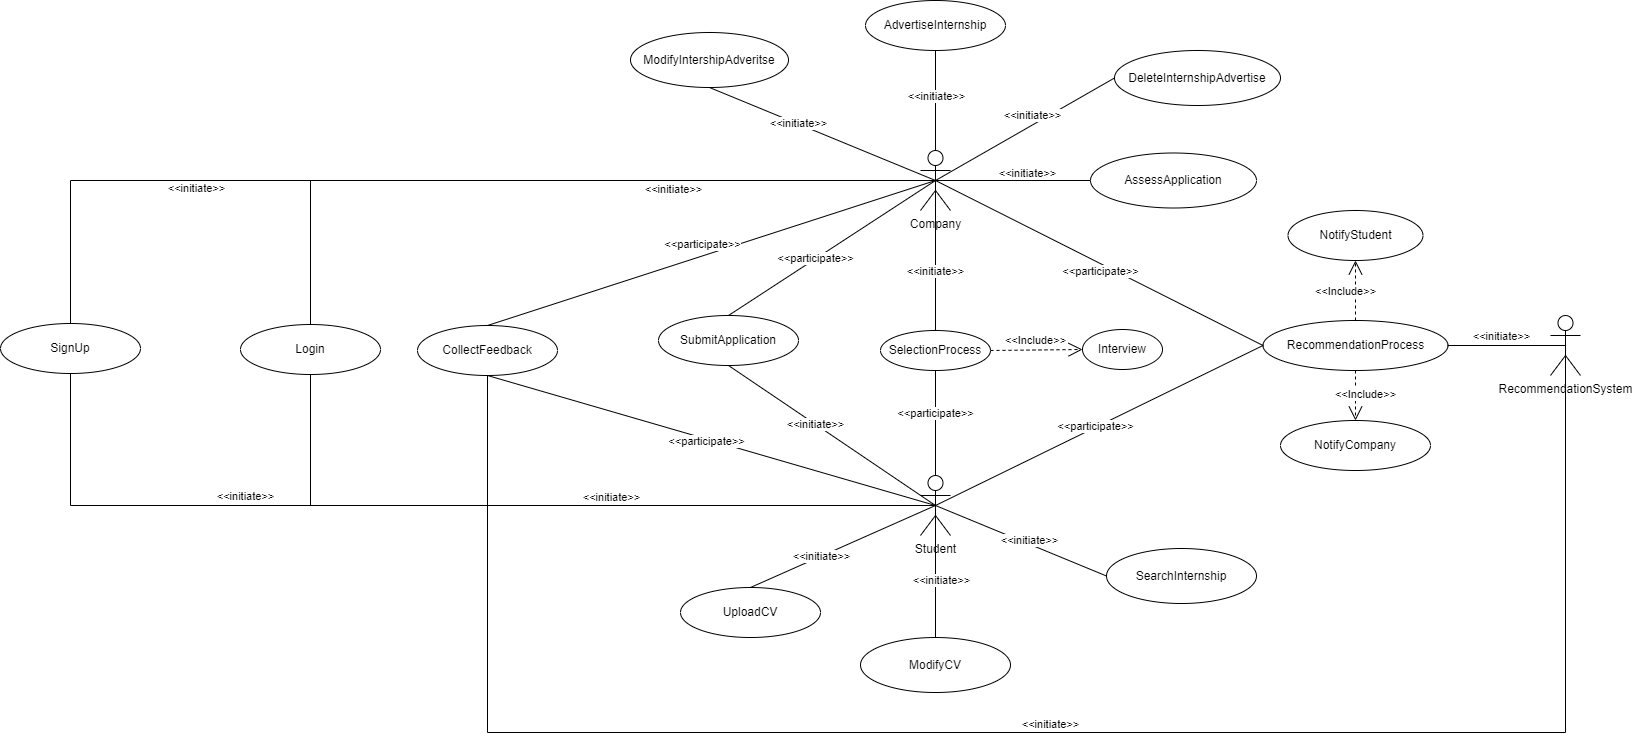
\includegraphics[scale = 0.3]{rasd_diagrams/UseCaseDiagram_v_1_5.png}
        \caption{Use Case Diagram}
        \label{fig:use_case_diagram}
    \end{figure}
\newpage
\subsubsection{Use Cases and Sequence Diagrams}

    In this section the uses cases illustrated in diagram \ref{fig:use_case_diagram} are described in their details, through sequence diagrams and tables to better understand the flow.
    
    \textbf{[UC1] - Sign-Up}
    
        \begin{figure}[H]
            \centering
            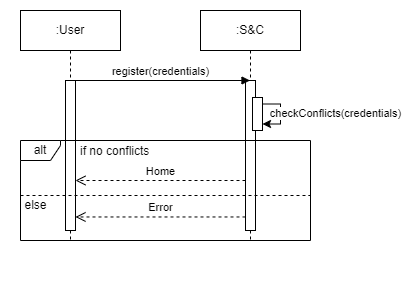
\includegraphics[scale = 0.7]{sequence_diagrams/SequenceDiagramSignUp_v_1_0.png}
            \caption{Sign-up sequence diagram}
            \label{fig:sign_up_sequence_diagram}
        \end{figure}
        
        \begin{center}
            \begin{longtable}{|l|p{0.75\linewidth}|}
                \hline
                \textbf{Name}
                & Sign-up \\
                \hline
                \textbf{Actors}
                & User (Student or Company) \\
                \hline
                \textbf{Entry Condition}
                & The user hasn't created an account yet. \\
                \hline
                \textbf{Event Flow}
                & 1 - User compiles the registration form. \\
                & 2 - User sends the form to S\&C platform which checks the information provided. \\
                \hline
                \textbf{Exit Condition}
                & If there are no conflicts in the user's info (for example, username already used), the registration process terminates correctly, and the homepage is sent to the user. \\
                \hline
                \textbf{Exception}
                   & \begin{itemize}
                        \item The user is already registered.
                        \item Conflicts in the information sent by the user.
                    \end{itemize} \\
                & An error message is shown to the user reporting the error. \\
                \hline
                \caption{Sign-up use case}
            \end{longtable}
        \end{center}
        
    \newpage
    
    \textbf{[UC2] - Log-in}
    
        \begin{figure}[H]
            \centering
            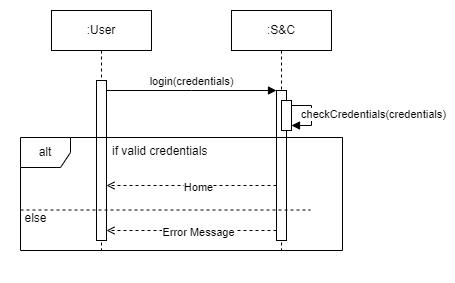
\includegraphics[scale = 0.7]{sequence_diagrams/SequenceDiagramLogin_v_1_0.png}
            \caption{Log-in sequence diagram}
            \label{fig:log_in_sequence_diagram}
        \end{figure}

        \begin{center}
            \begin{longtable}{|l|p{0.75\linewidth}|}
                \hline
                \textbf{Name}
                & Log-in \\
                \hline
                \textbf{Actors}
                & User (Student or Company) \\
                \hline
                \textbf{Entry Condition}
                & The user is registered but not logged in and tries to connect to the site URL. \\
                \hline
                \textbf{Event Flow}
                & 1 - User compiles the log-in form. \\
                & 2 - User sends the form to S\&C platform which checks the information provided. \\
                \hline
                \textbf{Exit Condition}
                & User's info are correct and the homepage is sent to the user. \\
                \hline
                \textbf{Exception}
                &  User's info don't match the ones stored in the database. \\
                \hline
                \caption{Log-in use case}
            \end{longtable}
        \end{center}

    \newpage
    
    \textbf{[UC3] - Upload CV}
    
        \begin{figure}[H]
            \centering
            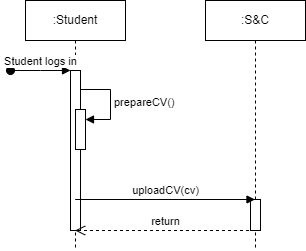
\includegraphics[scale = 0.7]{sequence_diagrams/SequenceDiagramUploadCV_v_1_1.png}
            \caption{Upload CV sequence diagram}
            \label{fig:upload_cv_sequence_diagram}
        \end{figure}

        \begin{center}
            \begin{longtable}{|l|p{0.75\linewidth}|}
                \hline
                \textbf{Name}
                & Upload CV \\
                \hline
                \textbf{Actors}
                & Student \\
                \hline
                \textbf{Entry Condition}
                & Student does not have a CV associated to his profile and logs into the site. \\
                \hline
                \textbf{Event Flow}
                & 1 - Student prepares his CV writing his experiences and personal information.\\
                & 2 - Student upload his CV to the platform. \\
                \hline
                \textbf{Exit Condition}
                & Student's CV is correctly uploaded on the platform. \\
                \hline
                \textbf{Exception}
                &  No exception \\
                \hline
                \caption{Upload CV use case}
            \end{longtable}
        \end{center}

    \newpage
    
    \textbf{[UC4] - Modify CV}
    
        \begin{figure}[H]
            \centering
            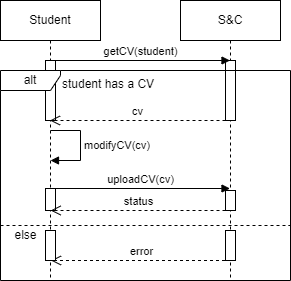
\includegraphics[scale = 0.7]{sequence_diagrams/SequenceDiagramModifyCV_v_1_0.png}
            \caption{Modify CV sequence diagram}
            \label{fig:modify_cv_sequence_diagram}
        \end{figure}

        \begin{center}
            \begin{longtable}{|l|p{0.75\linewidth}|}
                \hline
                \textbf{Name}
                & Modify CV \\
                \hline
                \textbf{Actors}
                & Student \\
                \hline
                \textbf{Entry Condition}
                & Student wants to modify his CV. \\
                \hline
                \textbf{Event Flow}
                & 1 - Student opens his CV.\\
                & 2 - Student modifies his CV. \\
                & 3 - Student uploads his modified CV to the platform. \\
                \hline
                \textbf{Exit Condition}
                & Student's CV is correctly modified and uploaded on the platform. \\
                \hline
                \textbf{Exception}
                &  Student does not possess a CV. \\
                \hline
                \caption{Modify CV use case}
            \end{longtable}
        \end{center}

    \newpage
        
    \textbf{[UC5] - Advertise internship}
    
        \begin{figure}[H]
            \centering
            
\includegraphics[scale = 0.7]{sequence_diagrams/SequenceDiagramAdvertiseInternship_v_1_0.png}
            \caption{Advertise internship sequence diagram}
            \label{fig:advertise_internship_sequence_diagram}
        \end{figure}

        \begin{center}
            \begin{longtable}{|l|p{0.75\linewidth}|}
                \hline
                \textbf{Name}
                & Advertise internship \\
                \hline
                \textbf{Actors}
                & Company \\
                \hline
                \textbf{Entry Condition}
                & Company logs is and wants to create an internship advertise. \\
                \hline
                \textbf{Event Flow}
                & 1 - Company clicks on "Create Internship".\\
                & 2 - Company compiles the "Create Internship Form" writing the project and possible terms\\
                & 3 - Company sends the form to S\&C. \\
                \hline
                \textbf{Exit Condition}
                & Internship advertise is published. \\
                \hline
                \textbf{Exception}
                &  No exception. \\
                \hline
                \caption{Advertise internship use case}
            \end{longtable}
        \end{center}

    \newpage
        
    \textbf{[UC6] - Modify internship advertise}
        \begin{figure}[H]
            \centering
            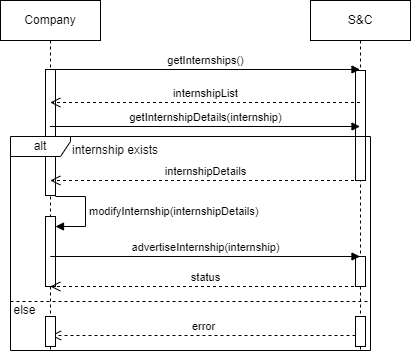
\includegraphics[scale = 0.7]{sequence_diagrams/SequenceDiagramModifyInternship_v_1_1.png}
            \caption{Modify internship advertise sequence diagram}
            \label{fig:modify_internship_sequence_diagram}
        \end{figure}

        \begin{center}
            \begin{longtable}{|l|p{0.75\linewidth}|}
                \hline
                \textbf{Name}
                & Modify internship \\
                \hline
                \textbf{Actors}
                & Company \\
                \hline
                \textbf{Entry Condition}
                & Company wants to modify its internship advertise. \\
                \hline
                \textbf{Event Flow}
                & 1 - Company choose which advertise to modify from the list of the company's advertises.\\
                & 2 - Company gets the details of the chosen advertise.\\
                & 3 - Company modifies the details of the chosen advertise. \\
                & 4 - Company sends the modified advertise back to S\&C. \\
                \hline
                \textbf{Exit Condition}
                & Modified internship advertise is published. \\
                \hline
                \textbf{Exception}
                & Internship details not available. \\
                \hline
                \caption{Modify internship use case}
            \end{longtable}
        \end{center}

    \newpage
        
    \textbf{[UC7] - Delete internship}
        \begin{figure}[H]
            \centering
            
\includegraphics[scale = 0.7]{sequence_diagrams/SequenceDiagramDeleteInternship_v_1_0.png}
            \caption{Delete internship sequence diagram}
            \label{fig:delete_internship_sequence_diagram}
        \end{figure}

        \begin{center}
            \begin{longtable}{|l|p{0.75\linewidth}|}
                \hline
                \textbf{Name}
                & Delete internship \\
                \hline
                \textbf{Actors}
                & Company \\
                \hline
                \textbf{Entry Condition}
                & Company wants to delete its internship advertise. \\
                \hline
                \textbf{Event Flow}
                & 1 - Company choose which advertise it wants to modify from the list of the company's advertises.\\
                & 2 - Company asks S\&C to delete the advertise.\\
                \hline
                \textbf{Exit Condition}
                & Internship advertise successfully deleted. \\
                \hline
                \textbf{Exception}
                & Internship advertise does not exist. \\
                \hline
                \caption{Delete internship use case}
            \end{longtable}
        \end{center}

    \newpage
        
    \textbf{[UC8] - Search internship}
    
        \begin{figure}[H]
            \centering
            
\includegraphics[scale = 0.7]{sequence_diagrams/SequenceDiagramSearchInternship_v_1_0.png}
            \caption{Search internship sequence diagram}
            \label{fig:search_internship_sequence_diagram}
        \end{figure}

        \begin{center}
            \begin{longtable}{|l|p{0.75\linewidth}|}
                \hline
                \textbf{Name}
                & Search internship \\
                \hline
                \textbf{Actors}
                & Student \\
                \hline
                \textbf{Entry Condition}
                & Student wants to search for internship advertise. \\
                \hline
                \textbf{Event Flow}
                & 1 - Student sets the search filters.\\
                & 2 - Student asks S\&C for advertises which satisfy the filters.\\
                \hline
                \textbf{Exit Condition}
                & S\&C sends the student the list of advertises. \\
                \hline
                \textbf{Exception}
                & No exception \\
                \hline
                \caption{Search internship use case}
            \end{longtable}
        \end{center}

    \newpage
        
    \textbf{[UC9] - Notify student about recommended internship}
    
        \begin{figure}[H]
            \centering
            
\includegraphics[scale = 0.6]{RASD/sequence_diagrams/SequenceDiagramNotifyStudent_v_1_2.png}
            \caption{Notify student about recommended internship sequence diagram}
            \label{fig:notify_student_sequence_diagram}
        \end{figure}

        \begin{center}
            \begin{longtable}{|l|p{0.75\linewidth}|}
                \hline
                \textbf{Name}
                & Notify student about recommended internship \\
                \hline
                \textbf{Actors}
                & Student \\
                & Recommendation System \\
                & Company \\
                \hline
                \textbf{Entry Condition}
                & Company uploads a new internship advertise \\
                \hline
                \textbf{Event Flow}
                & 1 - Recommendation System gets all CVs from S\&C. \\ 
                & 2 - S\&C returns the list of all CVs. \\
                & 3 - Recommendation System analyses the internship advertise and the list of CVs, searching for possible matches. \\
                & 4 - For every found match, the recommendation system asks information about the student. \\
                \hline
                \textbf{Exit Condition}
                & Recommendation notifies about the match both the company and the student. \\
                \hline
                \textbf{Exception}
                & No exception. \\
                \hline
                \caption{Notify student about recommended companies use case}
            \end{longtable}
        \end{center}

    \textbf{[UC10] - Notify company about recommended student}
    
        \begin{figure}[H]
            \centering
            
\includegraphics[scale = 0.6]{RASD/sequence_diagrams/SequenceDiagramNotifyCompany_v_1_1.png}
            \caption{Notify company about recommended students sequence diagram}
            \label{fig:notify_company_sequence_diagram}
        \end{figure}

        \begin{center}
            \begin{longtable}{|l|p{0.75\linewidth}|}
                \hline
                \textbf{Name}
                & Notify company about recommended students \\
                \hline
                \textbf{Actors}
                & Student \\
                & Recommendation System \\
                & Company \\
                \hline
                \textbf{Entry Condition}
                & Student uploads or modifies CV. \\
                \hline
                \textbf{Event Flow}
                & 1 - Recommendation System asks S\&C all the available internships. \\ 
                & 2 - S\&C returns all the available internships. \\
                & 3 - Recommendation System analyses the possible matching between internships and CV. \\
                & 4 - For every found match the recommendation system asks S\&C the information about the company. \\
                \hline
                \textbf{Exit Condition}
                & Recommendation notifies about the match both the company and the student. \\
                \hline
                \textbf{Exception}
                & No exception. \\
                \hline
                \caption{Notify company about recommended students use case}
            \end{longtable}
        \end{center}

    \newpage
        
    \textbf{[UC11] - Submit application}
    
        \begin{figure}[H]
            \centering
            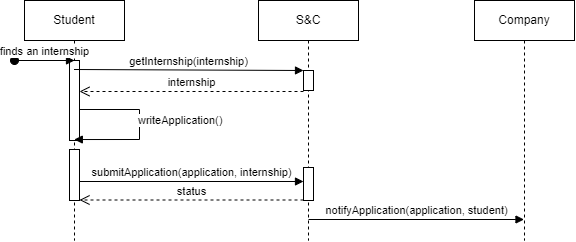
\includegraphics[scale = 0.7]{sequence_diagrams/SequenceDiagramSubmitApplication_v_1_2.png}
            \caption{Submit application sequence diagram}
            \label{fig:submit_application_sequence_diagram}
        \end{figure}

        \begin{center}
            \begin{longtable}{|l|p{0.75\linewidth}|}
                \hline
                \textbf{Name}
                & Submit application \\
                \hline
                \textbf{Actors}
                & Student \\
                & Company \\
                \hline
                \textbf{Entry Condition}
                & Student finds an internship he wants to apply to \\
                \hline
                \textbf{Event Flow}
                & 1 - Student asks for internship details to S\&C. \\ 
                & 2 - Student writes the application. \\
                & 3 - Student submits the application to the company through S\&C. \\
                & 4 - S\&C returns the status of the operation. \\
                \hline
                \textbf{Exit Condition}
                & Company receives the application from the student. \\
                \hline
                \textbf{Exception}
                & No exception. \\
                \hline
                \caption{Submit application use case}
            \end{longtable}
        \end{center}

    \newpage
        
    \textbf{[UC12] - Assess application}
    
        \begin{figure}[H]
            \centering
            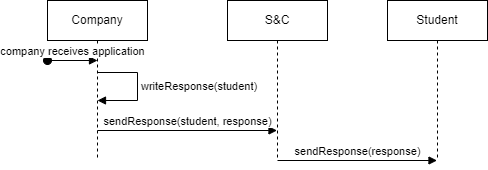
\includegraphics[scale = 0.7]{sequence_diagrams/SequenceAssessApplication_v_1_0.png}
            \caption{Assess application sequence diagram}
            \label{fig:assess_application_sequence_diagram}
        \end{figure}

        \begin{center}
            \begin{longtable}{|l|p{0.75\linewidth}|}
                \hline
                \textbf{Name}
                & Assess application \\
                \hline
                \textbf{Actors}
                & Student \\
                & Company \\
                \hline
                \textbf{Entry Condition}
                & Company receives an application from a student. \\
                \hline
                \textbf{Event Flow}
                & 1 - Company writes the response to the student. \\ 
                & 2 - Company sends the response through S\&C. \\
                \hline
                \textbf{Exit Condition}
                & Student receives the answer to his application. \\
                \hline
                \textbf{Exception}
                & No exception. \\
                \hline
                \caption{Assess application use case}
            \end{longtable}
        \end{center}

    \newpage
        
    \textbf{[UC13] - Collect feedback}
    
        \begin{figure}[H]
            \centering
            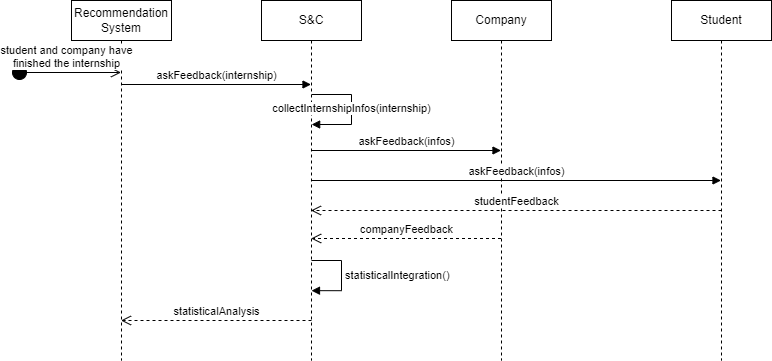
\includegraphics[scale = 0.7]{sequence_diagrams/SequenceDiagramCollectFeedback_v_1_1.png}
            \caption{Collect feedback sequence diagram}
            \label{fig:collect_feedback_sequence_diagram}
        \end{figure}

        \begin{center}
            \begin{longtable}{|l|p{0.75\linewidth}|}
                \hline
                \textbf{Name}
                & Collect feedback \\
                \hline
                \textbf{Actors}
                & Recommendation System \\
                & Student \\
                & Company \\
                \hline
                \textbf{Entry Condition}
                & Student and company have finished the internship period.\\
                \hline
                \textbf{Event Flow}
                & 1 - Recommendation system asks S\&C to collect feedback about a certain internship. \\
                & 2 - S\&C collects the internship details. \\
                & 3 - S\&C asks for feedback to both the company and the student involved in the internship. \\
                & 4 - Student and Company both provide their feedback to S\&C. \\
                & 5 - S\&C applies a statistical integrates the feedback with the stored data. \\
                \hline
                \textbf{Exit Condition}
                & Recommendation system receives the new statistical analysis to use to search for possible matches.\\
                \hline
                \textbf{Exception}
                & The company or the student does not provide feedback. \\
                \hline
                \caption{Collect feedback use case}
            \end{longtable}
        \end{center}

    \newpage
        
    \textbf{[UC14] - Selection process}
    
        \begin{figure}[H]
            \hspace*{-1.5cm}
            \centering
            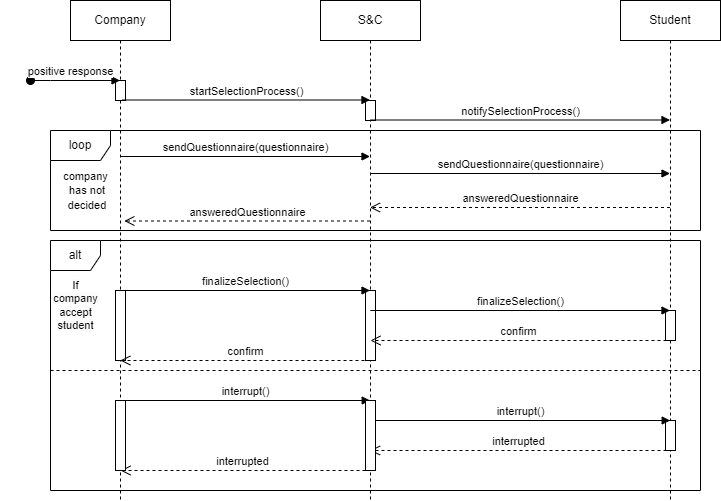
\includegraphics[scale = 0.7]{sequence_diagrams/SequenceDiagramSelectionProcess_v_1_1.png}
            \caption{Selection process sequence diagram}
            \label{fig:selection_process_sequence_diagram}
        \end{figure}
        
        \begin{center}
            \begin{longtable}{|l|p{0.75\linewidth}|}
                \hline
                \textbf{Name} & Selection process \\
                \hline
                \textbf{Actors} 
                & Company \\
                & Student \\
                \hline
                \textbf{Entry Condition}
                & Company has sent the student a positive response to their application. \\
                \hline
                \textbf{Event Flow}
                & 1 - Company starts the selection process and notifies student. \\
                & 2 - Company sends the student a questionnaire with the interview questions. \\
                & 3 - Student answers the questions and sends back the compiled questionnaire. \\
                & 4 - Company reads the response and decide wether the candidate is suited or not. \\
                & 5 - If the student is not suited return to step 2. \\
                \hline
                \textbf{Exit Condition}
                & If student is suited the student is hired and the selection process is closed. Otherwise the process is interrupted and the student is notified. \\
                \hline
                \textbf{Exception}
                & Student does not answer the questionnaires. \\
                \hline
                \caption{Selection process use case}
            \end{longtable}
        \end{center}

\newpage
\subsection{Performance Requirements}
    The system must be able to fulfill the requests of a great number of users simultaneously with a low response time, in order to maintain the overall experience as good as possible.
    It is worth to notice that if the user's connection is slow the response time would increase noticeably, regardless of the implementation. 
\subsection{Design Constraint}

\subsubsection{Standard compliance}
    There are no specific measures to adopt. The S\&C platform is subject to General Data Protection Regulation (GDPR), a regulation in EU law on data protection and privacy for all individuals within the European Union (EU) and European Economic Area (EAA).
\subsubsection{Hardware limitations}
    The only requirements to access and use S\&C are:
        \begin{itemize}
            \item A smartphone and/or a computer (of all operating system, such as Linux, Windows, Android etc.) with an updated browser to access the web app.
            \item A reliable internet connection to access the browser.
        \end{itemize}
\subsubsection{Any other constraint}
    There are no other particular constraints.
\subsection{Software System Attributes}

\subsubsection{Reliability}
    The system must be able to run without any interruption for a long period of time. To achieve so and in order to be fault tolerant, the system back-end must use some sort of replication and redundancy, as well as keeping an offline backup of the most important data, in case of failure.
    
\subsubsection{Availability}
    S\&C must provide an availability of 99\%, which means that the average downtime should be around 3.65 days/year. The system must avoid single point of failure and it has to be prepared to possibly large amount of data queried and uploaded. To achieve this, as stated above, the importance of replication and redundancy is underlined once again.

\subsubsection{Security}
    The system deals with sensitive information so the security aspect must be carefully considered. Password stored in S\&C databases must be encrypted. Seeing the type of sensitive data the implementation of 2-Factor-Access should be considered. Furthermore, to avoid sniffing and spoofing attacks, and guarantee the user's privacy, messages and data sent from client to server should be encrypted. 

\subsubsection{Maintainability}
    To ensure a good level of maintainability, the code has to be well documented. A test routine should provide functional coverage of at least 90\%. The user interface should be excluded from the tests.
    
\subsubsection{Portability}
    The system has to be compatible with different web browsers (e.g. Firefox, Chrome).
    
\section{Formal Analysis using Alloy}
    In this section we include a dynamic Alloy model for Student\&Companies underlining the following core aspects and features of the platform:

    \begin{itemize}
        \item Submission and evaluation of applications.
        \item Interview scheduling and student evaluation.
        \item Notification between company and students.
    \end{itemize}

\subsection{Signatures \& Functions}

    \begin{figure}[H]
        \centering
        
\includegraphics[width=\textwidth]{RASD/alloy/signature1.png}
        \label{fig:alloy_signature1}
    \end{figure}
    \begin{figure}[H]
        \centering
        
\includegraphics[width=\textwidth]{RASD/alloy/signature2.png}
        \label{fig:alloy_signature2}
    \end{figure}
    \begin{figure}[H]
        \centering
        
\includegraphics[width=\textwidth]{RASD/alloy/functions.png}
        \label{fig:alloy_functions}
    \end{figure}

\subsection{Facts}

    \begin{figure}[H]
        \centering
        
\includegraphics[width=\textwidth]{RASD/alloy/facts1.png}
        \label{fig:alloy_facts1}
    \end{figure}
    \begin{figure}[H]
        \centering
        
\includegraphics[width=\textwidth]{RASD/alloy/facts2.png}
        \label{fig:alloy_facts2}
    \end{figure}
    \begin{figure}[H]
        \centering
        
\includegraphics[width=\textwidth]{RASD/alloy/facts3.png}
        \label{fig:alloy_facts3}
    \end{figure}
    \begin{figure}[H]
        \centering
        
\includegraphics[width=\textwidth]{RASD/alloy/facts4.png}
        \label{fig:alloy_facts4}
    \end{figure}
    \begin{figure}[H]
        \centering
        
\includegraphics[width=\textwidth]{RASD/alloy/facts5.png}
        \label{fig:alloy_facts5}
    \end{figure}
    \begin{figure}[H]
        \centering
        
\includegraphics[width=\textwidth]{RASD/alloy/facts6.png}
        \label{fig:alloy_facts6}
    \end{figure}
    \begin{figure}[H]
        \centering
        
\includegraphics[width=\textwidth]{RASD/alloy/facts7.png}
        \label{fig:alloy_facts7}
    \end{figure}

\subsection{Predicates}

    \begin{figure}[H]
        \centering
        
\includegraphics[width=\textwidth]{RASD/alloy/predicates1.png}
        \label{fig:alloy_predicates1}
    \end{figure}
    \begin{figure}[H]
        \centering
        
\includegraphics[width=\textwidth]{RASD/alloy/predicates2.png}
        \label{fig:alloy_predicates2}
    \end{figure}
    \begin{figure}[H]
        \centering
        
\includegraphics[width=\textwidth]{RASD/alloy/predicates3.png}
        \label{fig:alloy_predicates3}
    \end{figure}

\subsection{Assertions \& Commands}
    
    \begin{figure}[H]
        \centering
        
\includegraphics[width=\textwidth]{RASD/alloy/assertions.png}
        \label{fig:alloy_assertions}
    \end{figure}
    \begin{figure}[H]
        \centering
        
\includegraphics[width=\textwidth]{RASD/alloy/commands.png}
        \label{fig:alloy_commands}
    \end{figure}
\newpage
\subsection{Results}
    \begin{figure}[H]
        \centering
        
\includegraphics[width=\textwidth]{RASD/alloy/results.png}
        \caption{Results}
        \label{fig:alloy_results}
    \end{figure}

\subsubsection{Generated world}

    \begin{figure}[H]
        \centering
        
\includegraphics[width=\textwidth]{RASD/alloy/world.png}
        \caption{Generated world}
        \label{fig:alloy_world}
    \end{figure}

\subsubsection{Predicate instances}
    
    \begin{figure}[H]
        \centering
        
\includegraphics[width=\textwidth]{RASD/alloy/studentapplies1.png}
        \caption{\textit{Studentapplies1} final state}
        \label{fig:alloy_studentapplies1}
    \end{figure}
    \begin{figure}[H]
        \centering
        
\includegraphics[width=\textwidth]{RASD/alloy/studentapplies2.png}
        \caption{\textit{Studentapplies2} final state}
        \label{fig:alloy_studentapplies2}
    \end{figure}
    \begin{figure}[H]
        \centering
        
\includegraphics[width=\textwidth]{RASD/alloy/studentapplies3.png}
        \caption{\textit{Studentapplies3} final state}
        \label{fig:alloy_studentapplies3}
    \end{figure}
\newpage
\section{Effort Spent}
In this section there is an overview of the time effort spent for each group member to write and revise each chapter of this document.
    \begin{itemize}
        \item \textbf{Davide Rodler}
            \begin{table}[H]
                \centering
                \begin{tabular}{|c|c|}
                    \hline
                    \textbf{Chapter} & \textbf{Effort (in hours)} \\
                    \hline
                    Chapter 1 &  5\\
                    \hline
                    Chapter 2 &  12\\
                    \hline
                    Chapter 3 &  15\\
                    \hline
                    Chapter 4 &  2\\
                    \hline
                \end{tabular}
            \end{table} 
      
        \item \textbf{Stefano Riva}
            \begin{table}[H]
                \centering
                \begin{tabular}{|c|c|}
                    \hline
                    \textbf{Chapter} & \textbf{Effort (in hours)} \\
                    \hline
                    Chapter 1 &  4\\
                    \hline
                    Chapter 2 &  3\\
                    \hline
                    Chapter 3 &  15\\
                    \hline
                    Chapter 4 &  15\\
                    \hline
                \end{tabular}
            \end{table}
    \end{itemize}

\section{Reference \& Used Tools}
\subsection{Paper References}
    \begin{itemize}
        \item Specification document 'Assignment RDD AY 2024-2025'.
        \item Slides from the Software Engineering 2 course.
    \end{itemize}
\subsection{Used Tools}
    \begin{itemize}
        \item Writing and Drafting the document: Overleaf.
        \item Diagrams drawing: Draw.io \& Visual Paradigm.
        \item Mock-ups mading: Canva.
        \item Alloy modeling and testing: Alloytools.
        \item Versioning: Github.
    \end{itemize}

\listoffigures
\newpage
\listoftables

\end{document}
